% !TeX program = xelatex
% ==========================================================================
%  本科毕业论文
%  题目：常微分方程初值问题的算法与应用
%  副题：IMEX 格式在 Burgers 方程上的耦合刚性稳定性
% ==========================================================================
\documentclass[UTF8,fontset=none,12pt,oneside,openany]{ctexbook}

% ---------- 页面与字体 ----------
\usepackage[a4paper,top=2.6cm,bottom=2.6cm,left=3.0cm,right=2.6cm,
            headheight=15pt,footskip=1.0cm]{geometry}
% 优先使用 Noto CJK；若系统未安装，则自动回退到 TeX Live 自带的 Fandol。
\IfFontExistsTF{Noto Serif CJK SC}
  {%
    \setCJKmainfont{Noto Serif CJK SC}[AutoFakeBold=2.0,AutoFakeSlant=0.2]
    \setCJKsansfont{Noto Sans CJK SC}[AutoFakeBold=2.0]
    \setCJKmonofont{Noto Sans Mono CJK SC}
  }
  {%
    \setCJKmainfont{FandolSong-Regular.otf}[BoldFont=FandolHei-Regular.otf,ItalicFont=FandolKai-Regular.otf]
    \setCJKsansfont{FandolHei-Regular.otf}
    \setCJKmonofont{FandolSong-Regular.otf}
  }
\setmainfont{TeX Gyre Termes}
\usepackage{unicode-math}
\setmathfont{TeX Gyre Termes Math}

% ---------- 数学与图表 ----------
\usepackage{amsmath,amsthm}
\usepackage{graphicx}
\usepackage{booktabs,multirow,array,tabularx,threeparttable}
\usepackage{enumitem}
\usepackage{xcolor}
\usepackage{tikz}
\usepackage[most]{tcolorbox}
\usepackage{listings}
\usepackage{caption}
\usepackage{float}
\usepackage{fancyhdr}

% ---------- 参考文献 ----------
\usepackage[backend=biber,style=gb7714-2015]{biblatex}
\addbibresource{refs.bib}

% ---------- 超链接 ----------
\usepackage[colorlinks=true,
            linkcolor=blue!55!black,
            citecolor=green!45!black,
            urlcolor=blue!65!black,
            bookmarksnumbered=true]{hyperref}

\hypersetup{
  pdftitle={常微分方程初值问题的算法与应用},
  pdfsubject={IMEX 格式在 Burgers 方程上的耦合刚性稳定性分析},
  pdfauthor={邹文杰},
  pdfkeywords={常微分方程初值问题, IMEX 格式, Burgers 方程, 耦合刚性, 稳定性函数, Jin-Xin 松弛},
  pdfcreator={XeLaTeX},
}

% ---------- 版式参数 ----------
\linespread{1.45}
\setlength{\parindent}{2em}
\setlength{\parskip}{0.15em}
\setcounter{secnumdepth}{3}
\setcounter{tocdepth}{2}
\allowdisplaybreaks
\numberwithin{equation}{chapter}

\ctexset{
  chapter = {
    name = {第,章},
    number = \chinese{chapter},
    beforeskip = 1.2\baselineskip,
    afterskip = 1.4\baselineskip,
  },
  section = {format = \Large\bfseries\sffamily},
  subsection = {format = \large\bfseries\sffamily},
  subsubsection = {format = \normalsize\bfseries\sffamily},
}

% ---------- 页眉页脚 ----------
\pagestyle{fancy}
\fancyhf{}
\fancyhead[L]{\small\sffamily\nouppercase{\leftmark}}
\fancyhead[R]{\small\sffamily 常微分方程初值问题的算法与应用}
\fancyfoot[C]{\small\thepage}
\renewcommand{\headrulewidth}{0.4pt}

% ---------- 图表标题 ----------
\captionsetup{font=small,labelfont=bf,labelsep=quad}
\captionsetup[table]{position=top,skip=6pt}
\captionsetup[figure]{skip=6pt}
\graphicspath{{figures/}}

% ---------- 定理环境 ----------
\theoremstyle{plain}
\newtheorem{theorem}{定理}[chapter]
\newtheorem{lemma}[theorem]{引理}
\newtheorem{proposition}[theorem]{命题}
\newtheorem{corollary}[theorem]{推论}
\theoremstyle{definition}
\newtheorem{definition}[theorem]{定义}
\newtheorem{example}[theorem]{例}
\theoremstyle{remark}
\newtheorem{remark}[theorem]{注}
\renewcommand{\proofname}{证明}

% ---------- 常用记号 ----------
\newcommand{\R}{\mathbb{R}}
\newcommand{\dd}{\mathrm{d}}
\newcommand{\bU}{{\mathbf{U}}}
\newcommand{\bA}{{\mathbf{A}}}
\newcommand{\bC}{{\mathbf{C}}}
\newcommand{\bD}{{\mathbf{D}}}
\newcommand{\bF}{{\mathbf{F}}}
\newcommand{\bI}{{\mathbf{I}}}
\newcommand{\bM}{{\mathbf{M}}}
\newcommand{\bL}{{\mathbf{L}}}
\newcommand{\bJ}{{\mathbf{J}}}
\newcommand{\bx}{{\boldsymbol{x}}}
\newcommand{\sgn}{\operatorname{sgn}}
\newcommand{\diag}{\operatorname{diag}}
\newcommand{\ee}{\mathrm{e}}
\newcommand{\ii}{\mathrm{i}}
\newcommand{\CFL}{\mathrm{CFL}}

% ---------- 代码样式 ----------
\lstset{
  basicstyle=\ttfamily\small,
  keywordstyle=\color{blue!70!black}\bfseries,
  commentstyle=\color{green!40!black},
  stringstyle=\color{red!55!black},
  numbers=left,
  numberstyle=\tiny\color{gray},
  frame=single,
  rulecolor=\color{gray!45},
  breaklines=true,
  columns=fullflexible,
  keepspaces=true,
  showstringspaces=false,
  captionpos=b,
}

% ==========================================================================
\begin{document}

% ==========================================================================
%  封面
% ==========================================================================
\begin{titlepage}
  \thispagestyle{empty}
  \begin{center}
    \vspace*{1.0cm}
    {\Large\sffamily 哈尔滨商业大学}\\[0.35cm]
    {\large\sffamily 本科毕业论文（设计）}\\[0.55cm]
    {\color{blue!45!black}\rule{\textwidth}{1.2pt}}\\[1.15cm]
    {\fontsize{25}{33}\selectfont\bfseries 常微分方程初值问题的算法与应用}\\[0.75cm]
    {\fontsize{15.5}{21}\selectfont\bfseries
      ——IMEX 格式在 Burgers 方程上的\\[0.18cm]
      耦合刚性稳定性分析}\\[0.55cm]
    {\color{blue!45!black}\rule{\textwidth}{0.6pt}}\\[2.1cm]
    \begin{tabular}{rl}
      {\sffamily 学\hspace{2em}院} & 基础科学学院 \\[0.38cm]
      {\sffamily 专\hspace{2em}业} & 数学与应用数学 \\[0.38cm]
      {\sffamily 学\hspace{2em}号} & 202336020064 \\[0.38cm]
      {\sffamily 姓\hspace{2em}名} & 邹文杰 \\[0.38cm]
      {\sffamily 指导教师} & 任中贵 \\[0.38cm]
    \end{tabular}
    \vfill
    {\large 二〇二六年十一月}
  \end{center}
\end{titlepage}


\frontmatter
\pagestyle{plain}

% ==========================================================================
%  中英文摘要
% ==========================================================================
\chapter*{\texorpdfstring{摘\quad 要}{摘要}}
\addcontentsline{toc}{chapter}{摘要}
\markboth{摘要}{}

\begingroup
\linespread{1.28}\selectfont

常微分方程初值问题的数值求解是科学与工程计算的基础。当右端函数含有多个时间尺度时，问题呈现刚性：显式方法受稳定性约束，隐式方法每步需要求解非线性方程组。IMEX（隐式—显式）方法对刚性部分采用隐式、对非刚性部分采用显式，在保持稳定性的同时显著降低计算量，是刚性初值问题的一类重要算法。本文以一维粘性 Burgers 方程为例，通过一阶有限体积方法与直线法将其转化为半离散刚性初值问题，系统研究参数化 IMEX-Euler 分裂族的耦合刚性稳定性。

本文引入分裂参数 $\theta\in[0,1]$，将耗散算子按 $\theta$ 与 $1-\theta$ 的比例分配至显式与隐式部分，得到覆盖全显式（$\theta=1$）、对半分裂（$\theta=1/2$）与全隐式（$\theta=0$）的分裂族。针对线性化模型，本文定义双变量稳定性函数
\[
  R(z_E,z_I)=\frac{1+z_E}{1-z_I},
\]
把稳定性问题化为复平面上的一族圆盘与一条耦合刚性射线的位置关系。本文证明：在耗散主导的耦合刚性极限下，$|R|\le 1$ 当且仅当 $\theta\le 1/2$；更精确地，当 $\theta>1/2$ 时，仅当 $|z_D|\le 2/(2\theta-1)$ 时格式稳定。进一步给出连续符号下的联合稳定条件 $\mu^2\le 2d+(1-2\theta)d^2$，并用刚性比 $\varepsilon=z_I/z_E$ 把判据写成 $|\varepsilon|\ge1$。分析表明，只有 $\theta=0$ 是 L-稳定的，$\theta=1/2$ 为临界稳定但不具有刚性衰减。离散 Fourier 符号分析给出了与理论一致的 CFL 型条件，并解释了数值实验中出现的网格尺度不稳定机制。

数值方面，本文在 Burgers 激波算例上完成了四组实验：固定 CFL 扫描黏性系数的刚性相图、不同 $\theta$ 下的最大稳定步长、激波位置与过渡层厚度的定量比较，以及网格收敛性测试。实验结果与理论预测一致：$\theta\le 1/2$ 时格式在刚性极限下保持稳定；$\theta>1/2$ 时最大稳定步长按 $O(\Delta x^2/\nu)$ 收缩，实测与线性预测相差不超过 $2\%$。MUSCL/minmod 重构使 $L^1$ 误差降低 $15$ 至 $28$ 倍，观测收敛阶约为 $2$。

作为扩展，本文将上述语言用于 Burgers 方程对应的 Jin--Xin 松弛系统，比较源项全隐式（策略 A）与仅隐式化线性刚性部分（策略 B）两种分裂。谱分析表明，策略 A 在 $\CFL\le 1$ 时稳定，策略 B 的容许 CFL 上限为 $1/3$，且该限制不随 $\varepsilon\to 0$ 而消失；数值实验验证了策略 B 在 $\CFL=0.7$ 时的失稳。本文的分析框架与代码流程可迁移至更一般的双曲守恒律与刚性松弛系统。

\vspace{1.2em}
\noindent{\bfseries 关键词：}常微分方程初值问题；IMEX 格式；Burgers 方程；耦合刚性；双变量稳定性函数；Jin--Xin 松弛
\endgroup

\clearpage

\chapter*{\texorpdfstring{Abstract}{Abstract}}
\addcontentsline{toc}{chapter}{Abstract}
\markboth{Abstract}{}

\begingroup
\linespread{1.08}\selectfont

Initial value problems (IVPs) for ordinary differential equations (ODEs) are a central object of numerical analysis. When several time scales are present, the IVP is stiff: explicit methods are restricted by stability, while fully implicit methods require a nonlinear solve at every step. Implicit--explicit (IMEX) schemes treat the stiff part implicitly and the non-stiff part explicitly, retaining stability at a reduced computational cost. Taking the one-dimensional viscous Burgers equation as a model, this thesis converts it, by a first-order finite-volume method and the method of lines, into a semi-discrete stiff IVP, and systematically studies the coupled-stiff stability of a parameterised IMEX--Euler family.

A splitting parameter $\theta\in[0,1]$ distributes the diffusion operator between the explicit and implicit parts, covering fully explicit ($\theta=1$), half-and-half ($\theta=1/2$) and fully implicit ($\theta=0$) splittings. For the linearised model, a two-variable stability function
\[
  R(z_E,z_I)=\frac{1+z_E}{1-z_I}
\]
is introduced, which reduces stability to the position of a coupled stiff ray relative to a family of disks in the complex plane. It is proved that $|R|\le 1$ in the diffusion-dominated coupled stiff limit if and only if $\theta\le 1/2$; more precisely, for $\theta>1/2$ stability holds only when $|z_D|\le 2/(2\theta-1)$. A joint stability condition $\mu^2\le 2d+(1-2\theta)d^2$ is derived for the continuous symbol, and the criterion is recast as $|\varepsilon|\ge1$ with the stiffness ratio $\varepsilon=z_I/z_E$. Only $\theta=0$ is L-stable, whereas $\theta=1/2$ is marginally stable but lacks stiff decay. A discrete Fourier symbol analysis yields consistent CFL-type conditions and explains the grid-scale instability observed in the numerical experiments.

Numerical experiments on a Burgers shock include a stiffness phase diagram, maximum stable time steps, and quantitative comparisons of the shock position, the transition-layer thickness and the $L^1$ error. The results agree with the theory: $\theta\le 1/2$ remains stable in the stiff limit, while for $\theta>1/2$ the maximal step scales like $O(\Delta x^2/\nu)$. The MUSCL/minmod reconstruction reduces the $L^1$ error by a factor of $15$--$28$, with an observed order close to two.

As an extension, the same framework is applied to the Jin--Xin relaxation system for Burgers' equation. Two source splittings are compared: a fully implicit one (strategy A) and a linearly implicit one (strategy B). Spectral analysis shows that A is stable for $\CFL\le 1$, whereas B admits only $\CFL\le 1/3$, a restriction that does not disappear as $\varepsilon\to0$; numerical experiments confirm the instability of B at $\CFL=0.7$. The analysis and the code flow are transferable to more general hyperbolic conservation laws with stiff relaxation.

\vspace{1.2em}
\noindent{\bfseries Keywords:} initial value problem for ODEs; IMEX scheme; Burgers equation; coupled stiffness; two-variable stability function; Jin--Xin relaxation
\endgroup


\tableofcontents
\cleardoublepage
\pagestyle{fancy}

\mainmatter
\pagestyle{fancy}

% ==========================================================================
\chapter{绪论}
\pagestyle{fancy}
% ==========================================================================

\section{研究背景与意义}

常微分方程初值问题
\begin{equation}
  \frac{\dd y}{\dd t}=f(t,y),\qquad y(t_0)=y_0,
  \label{eq:ode-ivp}
\end{equation}
是数值分析中最基本的模型问题之一。无论是化学反应动力学、电路仿真、生物网络，还是偏微分方程经过空间离散后得到的半离散系统，最终都归结为形如 \eqref{eq:ode-ivp} 的初值问题。对于这类问题，数值方法的研究围绕三个相互牵制的目标展开：精度、稳定性和计算效率。显式方法（如显式 Euler、显式 Runge--Kutta）每步只需计算若干次右端函数，实现简单，但其稳定域有界；隐式方法（如隐式 Euler、Gear 方法）具有更好的稳定性，但每步需要求解线性或非线性方程组。当问题同时含有快、慢两种时间尺度时，这种矛盾尤为突出。

这种多尺度特征通常用“刚性”（stiffness）来刻画。粗略地说，若微分方程的解由缓慢变化的模态主导，而扰动中却含有衰减极快的模态，则问题是刚性的。以线性常系数系统 $y'=Ay$ 为例，若 Jacobian 矩阵 $A$ 的特征值实部均为负，且最大与最小模长之比很大，则称问题是刚性的。刚性带来的困难并不在于解的性态复杂，而在于显式方法的稳定步长被最快的衰减模态所限制，尽管该模态在解中几乎不可见。隐式方法虽然可以放宽这一限制，却牺牲了每步的计算简便性。

IMEX（implicit--explicit，隐式—显式）方法正是在这一背景下发展起来的一类分裂时间推进格式。其基本思想是把右端算子分裂为刚性部分与非刚性部分：对刚性部分采用隐式处理以保证稳定性，对非刚性部分采用显式处理以控制计算量。以本文考虑的半离散系统
\begin{equation}
  \frac{\dd \bU}{\dd t}=\bC(\bU)+\nu\bD\bU
  \label{eq:semidiscrete-intro}
\end{equation}
为例，其中 $\bC$ 为对流算子，$\nu\bD$ 为耗散算子，IMEX-Euler 格式为
\begin{equation}
  \frac{\bU^{n+1}-\bU^{n}}{\Delta t}
  =\bC(\bU^{n})+\nu\bD\bU^{n+1}.
  \label{eq:imex-euler-intro}
\end{equation}
每一步只需解一个线性方程组，既避免了对流项的隐式非线性迭代，又消除了扩散项的显式稳定性限制。这类格式在反应扩散方程、大气模拟、等离子体输运和 Kinetic 方程中都有广泛应用。

本文的研究对象是上述思想的一个具体而富有代表性的实例：一维粘性 Burgers 方程
\begin{equation}
  u_t+\left(\frac{u^2}{2}\right)_x=\nu u_{xx},\qquad \nu>0.
  \label{eq:burgers-intro}
\end{equation}
Burgers 方程是 Navier--Stokes 方程的一维简化模型，既保留了对流项的非线性与激波形成机制，又包含了扩散项的光滑化作用。它的粘性激波具有显式解析解，便于对数值格式进行定量检验。因此，它常被用作检验双曲型数值方法的“标准试金石”。

从常微分方程初值问题的角度看，对 \eqref{eq:burgers-intro} 作空间有限体积离散并采用直线法（method of lines, MOL），可得形如 \eqref{eq:semidiscrete-intro} 的大型刚性初值问题。其 Jacobian 的特征值中，对流部分量级为 $O(1/\Delta x)$，扩散部分量级为 $O(\nu/\Delta x^2)$。当网格加密时，扩散特征值的模迅速增大，刚性比随之发散。因此，Burgers 方程恰好提供了一个可以精确控制刚性强弱、又可以与解析解比较的试验平台。

本文不局限于某一个固定的分裂方式，而是引入分裂参数 $\theta\in[0,1]$，把耗散算子按比例分配到显式与隐式部分：
\begin{equation}
  \frac{\dd \bU}{\dd t}
  =\bC(\bU)+\theta\nu\bD\bU+(1-\theta)\nu\bD\bU,
  \label{eq:theta-family-intro}
\end{equation}
其中前两项（对流项与比例为 $\theta$ 的耗散项）作显式处理，最后一项（比例为 $1-\theta$ 的耗散项）作隐式处理。$\theta=1$ 对应耗散全显式，$\theta=0$ 对应耗散全隐式，$\theta=1/2$ 对应耗散对半分配。这个单参数族把“全显式”和“全隐式”两个端点用一条连续路径连接起来，使得我们可以系统地回答如下问题：在什么条件下，一个分裂是“容许”的？稳定性边界由什么决定？稳定性与精度之间如何权衡？

研究这一问题的意义有两方面。理论上，它把常微分方程稳定性理论中的 A-稳定、L-稳定等概念，推广到“双变量稳定性函数”的框架中，为分析分裂型 IMEX 格式提供了一个统一的几何图像。实践上，所得判据可以直接指导参数选择与时间步长控制，并为后续研究高维双曲守恒律、松弛系统和动理学方程提供可迁移的方法与代码基础。

\section{国内外研究现状}

\subsection{IMEX 时间推进方法}

IMEX 方法的思想可以追溯到 Crouzeix 在 1980 年提出的隐式—显式线性多步法\cite{crouzeix1980}。20 世纪 90 年代以后，随着对流扩散、反应扩散等问题的大规模计算需求，IMEX Runge--Kutta 方法得到系统发展。Ascher、Ruuth 和 Spiteri 在 1997 年构造了面向时变偏微分方程的一类 IMEX Runge--Kutta 格式，并给出阶条件与稳定性分析\cite{ascher1997}。Pareschi 和 Russo 将 IMEX Runge--Kutta 方法应用于带刚性松弛的双曲系统，强调了渐近保持性质\cite{pareschi2005}。Boscarino 则从微分代数方程的角度分析了 IMEX 方法的误差传播与阶退化现象\cite{boscarino2007}。2024 年，Boscarino 与 Russo 对拟线性双曲系统的渐近保持方法作了系统综述\cite{boscarino2024}，其中对源项分裂、刚性极限和容许性条件的讨论，构成了本文重要的方法论背景。

国内学者在 IMEX 方法及其应用方面也有大量工作，研究范围覆盖对流扩散方程、浅水方程、多相流和动理学方程等。总体而言，现有研究多针对某一具体格式或某一类方程，对“分裂参数如何影响稳定性”这一设计层面的问题，系统性的参数化分析仍不多见。

\subsection{刚性与稳定性理论}

刚性常微分方程的稳定性理论奠基于 Dahlquist 关于线性多步法 A-稳定的经典工作\cite{dahlquist1963}。A-稳定要求方法的绝对稳定域包含整个左半复平面；L-稳定进一步要求放大因子在 $\mathrm{Re}\,z\to-\infty$ 时趋于零，从而对最快的衰减模态具有“刚性衰减”作用。Hairer 与 Wanner 的专著\cite{hairer1996}对刚性问题的理论、算法与实现作了全面总结。Gear 的早期工作\cite{gear1971}则奠定了刚性积分器的实践基础。

对于分裂型 IMEX 格式，稳定性不再由单个复变量 $z$ 描述，而需要同时考虑显式部分与隐式部分的贡献。设 $\lambda_E$ 与 $\lambda_I$ 分别为显式、隐式算子的特征值，令 $z_E=\Delta t\lambda_E$，$z_I=\Delta t\lambda_I$，则 IMEX-Euler 的放大因子为
\begin{equation}
  R(z_E,z_I)=\frac{1+z_E}{1-z_I}.
  \label{eq:R-intro}
\end{equation}
这一双变量稳定性函数是本文的核心工具。Zakerzadeh 与 Noelle 在 2018 年针对刚性双曲守恒律的 IMEX 通量分裂，比较了对称分裂与非对称分裂的稳定性：对称分裂可以做到对刚性参数一致稳定，而非对称分裂必须逐个检验，他们并给出了存在小范围不稳定区域的反例\cite{zakerzadeh2018}。本文将这一思想具体化为耗散算子的按比例分裂，并给出精确的有限刚性稳定性边界。

\subsection{有限体积方法与直线法}

本文的空间离散采用一阶有限体积方法。有限体积方法以守恒形式为出发点，直接对单元平均值进行演化，天然保证离散守恒性。Godunov 在 1959 年提出的迎风格式\cite{godunov1959}和 Rusanov 在 1961 年提出的局部 Lax--Friedrichs 通量\cite{rusanov1961}，是两类最基础的数值通量。van Leer 的 MUSCL 重构\cite{vanleer1979}通过斜率限制器把格式推广到二阶，同时保持总变差有界（TVD）。LeVeque 的专著\cite{leveque2002}与 Toro 的专著\cite{toro2009}对有限体积方法的理论、通量构造和激波捕捉作了系统阐述。

直线法把空间离散与时间推进分离：先对半离散系统 \eqref{eq:semidiscrete-intro} 选用 ODE 求解器，再单独分析时间格式的稳定性。这种模块化结构正是本文代码设计的基础，也使得常微分方程初值问题的算法分析可以直接服务于偏微分方程的数值模拟。

\subsection{松弛系统与渐近保持格式}

Jin 与 Xin 在 1995 年提出了用于双曲守恒律的松弛格式\cite{jinxin1995}：用一个线性双曲系统加刚性源项逼近非线性守恒律，当松弛参数 $\varepsilon\to0$ 时恢复到原方程。该框架的优点是通量线性化，便于构造高分辨率格式；代价是源项具有 $1/\varepsilon$ 的刚性，必须采用隐式或渐近保持（asymptotic preserving, AP）处理。Jin 随后系统发展了 AP 格式的理论\cite{jin1999}，Dimarco 与 Pareschi 则对动理学方程的数值方法作了综述\cite{dimarco2014}。

在松弛系统中，源项分裂方式直接决定了格式的稳定性与渐近相容性。全隐式源项通常具有最好的稳定性，但每步需要求解耦合方程；只隐式化线性刚性部分、把非线性部分显式处理，则可以降低实现难度，却可能破坏容许性。本文将在第六章用双变量稳定性函数的语言，对这两种分裂作系统比较。

\section{本文主要工作}

围绕“参数化分裂族的耦合刚性稳定性”这一主题，本文完成了以下工作。

第一，建立了一个覆盖全显式到全隐式的单参数分裂族。引入 $\theta\in[0,1]$，把耗散算子按 $\theta$ 与 $1-\theta$ 分配至显式与隐式部分，并以 IMEX-Euler 作为时间推进格式。该族把常见的三种分裂（全显式、对半、全隐式）纳入同一分析框架。

第二，定义了双变量稳定性函数 $R(z_E,z_I)$，并给出了耦合刚性极限的精确刻画。对线性化模型 $u_t+au_x=\nu u_{xx}$，在耗散主导、对流可忽略的极限下，证明 $|R|\le1$ 当且仅当 $\theta\le1/2$；更精确地，当 $\theta>1/2$ 时，稳定当且仅当 $|z_D|\le2/(2\theta-1)$。本文还给出两种证明：代数证明与复平面圆盘的几何证明。进一步区分了 A-稳定与 L-稳定：只有 $\theta=0$ 具有刚性衰减，$\theta=1/2$ 是临界情形。

第三，完成了离散 Fourier 符号分析。对一阶 Rusanov 通量，导出放大因子并给出 CFL 型条件；通过网格尺度（$\xi=\pi$）分析，解释了 $\theta>1/2$ 时最大稳定步长按 $O(\Delta x^2/\nu)$ 收缩的机制。分析同时表明，Rusanov 通量自带的数值扩散会略微放宽稳定域，但在 $\Delta x\to0$ 时该效应消失，理论边界是尖锐的。

第四，设计并完成了四组数值实验：固定 CFL 下的刚性相图、不同 $\theta$ 下的最大稳定步长扫描、粘性激波的精度测试，以及网格收敛性测试。实验采用一阶 Rusanov 通量与 MUSCL/minmod 重构两种空间格式，输出激波位置误差、过渡层厚度和 $L^1$ 误差。实验结果与理论预测一致，并揭示了“稳定”与“准确”并不等价：$\theta=1/2$ 是稳定性的临界点，却不是精度最优的选择。

第五，将上述框架扩展到 Burgers 方程对应的 Jin--Xin 松弛系统。比较了源项全隐式（策略 A）与仅隐式化线性刚性部分（策略 B）两种分裂，推导了 $2\times2$ 放大矩阵，并通过谱半径扫描得到：策略 A 在 $\CFL\le1$ 时稳定；策略 B 的容许 CFL 上限为 $1/3$，且该限制不随 $\varepsilon\to0$ 而消失。数值实验验证了策略 B 在 $\CFL=0.7$ 时的失稳。

本文的方法论价值在于：把“容许分裂”“双变量稳定性函数”“耦合刚性极限”“L-稳定”这套语言，落实为一个可以计算、可以作图、可以用数值实验检验的完整流程。代码采用 Python 实现，结构清晰，可直接迁移到其他双曲守恒律与松弛系统。

\section{论文结构}

全文共七章，安排如下。

第一章为绪论，介绍研究背景、国内外现状、本文工作与结构。

第二章为预备知识，回顾常微分方程初值问题的基本算法与刚性概念，介绍 A-稳定、L-稳定、von Neumann 分析、有限体积方法与直线法，并给出 IMEX-Euler 的推导与双变量稳定性函数的初步定义。

第三章建立模型与分裂族，推导粘性 Burgers 方程的有限体积半离散系统，引入参数化分裂族，说明 IMEX-Euler 的实现细节与离散参数。

第四章是稳定性分析的核心，定义双变量稳定性函数与容许分裂，证明 $\theta\le1/2$ 的充要条件，讨论 L-稳定与离散符号修正。

第五章为数值验证，介绍实验设计，给出刚性相图、最大稳定步长、激波精度与收敛性结果，并讨论稳定性与精度的关系。

第六章为扩展，研究 Jin--Xin 松弛系统的两种源项分裂，推导放大矩阵，比较刚性极限行为，并做数值对比。

第七章总结全文，指出局限性与后续研究方向。

附录给出核心代码片段与复现说明。

% ==========================================================================
\chapter{预备知识}
% ==========================================================================

本章回顾论文所需的基础知识。偏微分方程的理论基础可参阅文献\cite{zhou2005}。第 \ref{sec:ode-stiff} 节从常微分方程初值问题出发，介绍刚性概念与几类基本算法；第 \ref{sec:stability} 节整理 A-稳定、L-稳定等稳定性概念；第 \ref{sec:von-neumann} 节介绍 von Neumann 分析方法；第 \ref{sec:fv-mol} 节介绍有限体积方法与直线法；第 \ref{sec:imex-basic} 节给出 IMEX-Euler 的推导与双变量稳定性函数的初步定义。

\section{常微分方程初值问题与刚性}
\label{sec:ode-stiff}

考虑初值问题 \eqref{eq:ode-ivp}。假设 $f:\R\times\R^m\to\R^m$ 关于 $y$ 满足 Lipschitz 条件，则由 Picard--Lindel\"of 定理，问题在局部存在唯一解。数值方法的目标是构造离散时刻 $t_n$ 上的近似值 $y_n$，使得当步长 $\Delta t\to0$ 时，整体误差以预期的阶数趋于零。

最简单的两种方法是显式 Euler 法与隐式 Euler 法：
\begin{align}
  y_{n+1} &= y_n+\Delta t\,f(t_n,y_n), \label{eq:explicit-euler}\\
  y_{n+1} &= y_n+\Delta t\,f(t_{n+1},y_{n+1}). \label{eq:implicit-euler}
\end{align}
显式 Euler 法是一阶单步法，每步只需一次函数求值；隐式 Euler 法也是一阶，但每步需要解方程 \eqref{eq:implicit-euler}。当 $f$ 关于 $y$ 非线性时，通常采用 Newton 迭代；当 $f$ 线性时，则化为线性方程组。梯形法则
\begin{equation}
  y_{n+1}=y_n+\frac{\Delta t}{2}\bigl[f(t_n,y_n)+f(t_{n+1},y_{n+1})\bigr]
  \label{eq:trapezoidal}
\end{equation}
是二阶的，但它对刚性模态的衰减不够强，这一点将在第 \ref{sec:stability} 节说明。

\subsection{刚性的含义}

“刚性”并没有一个完全统一的定义，但其核心是时间尺度的分离。对线性系统
\begin{equation}
  y'=Ay,\qquad A\in\R^{m\times m},
  \label{eq:linear-system}
\end{equation}
设 $A$ 的特征值为 $\lambda_1,\dots,\lambda_m$，且 $\mathrm{Re}\,\lambda_j<0$。若
\begin{equation}
  S=\frac{\max_j|\mathrm{Re}\,\lambda_j|}{\min_j|\mathrm{Re}\,\lambda_j|}\gg1,
  \label{eq:stiffness-ratio}
\end{equation}
则称系统是刚性的，$S$ 称为刚性比。对非线性问题，可以用 Jacobian 矩阵 $f_y(t,y)$ 的特征值作局部化的定义。

刚性带来的困难可以通过一个简单例子说明。取
\begin{equation}
  y'=-1000\bigl(y-\cos t\bigr)-\sin t,\qquad y(0)=1,
  \label{eq:stiff-example}
\end{equation}
其精确解为 $y(t)=\cos t$。该问题的 Jacobian 为 $-1000$，快模态以时间尺度 $10^{-3}$ 衰减，而解本身以 $O(1)$ 的尺度变化。表 \ref{tab:stiff-example} 给出了显式 Euler 与隐式 Euler 在不同步长下的最大误差。

\begin{table}[htbp]
  \centering
  \caption{刚性初值问题 \eqref{eq:stiff-example} 的数值结果（$t\in[0,1]$）}
  \label{tab:stiff-example}
  \begin{tabular}{lccc}
    \toprule
    方法 & 步长 $\Delta t$ & 最大误差 & 是否稳定 \\
    \midrule
    显式 Euler & $1.0\times10^{-3}$ & $5.00\times10^{-7}$ & 是 \\
    显式 Euler & $2.0\times10^{-3}$ & $2.00\times10^{-6}$ & 是 \\
    显式 Euler & $2.1\times10^{-3}$ & 发散 & 否 \\
    \midrule
    隐式 Euler & $1.0\times10^{-2}$ & $8.39\times10^{-3}$ & 是 \\
    隐式 Euler & $5.0\times10^{-2}$ & $4.14\times10^{-2}$ & 是 \\
    隐式 Euler & $1.0\times10^{-1}$ & $8.13\times10^{-2}$ & 是 \\
    \bottomrule
  \end{tabular}
\end{table}

显式 Euler 的稳定条件是 $|1-1000\Delta t|\le1$，即 $\Delta t\le2\times10^{-3}$；一旦越过该阈值，误差迅速放大。隐式 Euler 对任意 $\Delta t>0$ 都稳定，但步长增大时精度下降。这一对比揭示了刚性问题的基本矛盾：稳定性要求与精度要求往往指向不同的步长。IMEX 方法试图在两者之间取得平衡：把导致刚性限制的项隐式处理，把其余项显式处理。

\subsection{从偏微分方程到刚性初值问题}

直线法把偏微分方程的空间变量离散，得到一个关于时间的大型常微分方程组。以一维对流扩散方程
\begin{equation}
  u_t+a u_x=\nu u_{xx}
  \label{eq:adv-diff}
\end{equation}
为例，若用中心差分离散空间导数，得到
\begin{equation}
  \frac{\dd u_j}{\dd t}
  =-a\frac{u_{j+1}-u_{j-1}}{2\Delta x}
  +\nu\frac{u_{j+1}-2u_j+u_{j-1}}{\Delta x^2}.
  \label{eq:adv-diff-semi}
\end{equation}
对 Fourier 模态 $u_j=\hat u\ee^{\ii kx_j}$，右端符号为
\begin{equation}
  \lambda(k)=-\ii ak-\nu k^2.
  \label{eq:adv-diff-symbol}
\end{equation}
在网格可分辨的波数范围内，$|k|\le\pi/\Delta x$，因此对流特征值的模为 $O(a/\Delta x)$，扩散特征值的模为 $O(\nu/\Delta x^2)$。当 $\Delta x\to0$ 时，扩散特征值增长得更快，刚性比 $S=O(\nu/(a\Delta x))\to\infty$。这说明：即使原偏微分方程并不“刚性”，空间离散也会把刚性引入半离散系统。对 Burgers 方程，这一机制同样成立，只是对流项变成了非线性。

\section{稳定性概念}
\label{sec:stability}

\subsection{测试方程与放大因子}

线性稳定性分析通常以标量测试方程
\begin{equation}
  y'=\lambda y,\qquad \mathrm{Re}\,\lambda<0
  \label{eq:test-equation}
\end{equation}
为出发点。若数值方法作用在 \eqref{eq:test-equation} 上给出
\begin{equation}
  y_{n+1}=R(z)y_n,\qquad z=\Delta t\lambda,
  \label{eq:amplification}
\end{equation}
则 $R(z)$ 称为放大因子（或稳定性函数）。方法的绝对稳定域定义为
\begin{equation}
  \mathcal{S}=\{z\in\mathbb{C}: |R(z)|\le1\}.
  \label{eq:stability-region}
\end{equation}
显式 Euler 的 $R(z)=1+z$，稳定域是以 $-1$ 为圆心、半径为 $1$ 的圆盘；隐式 Euler 的 $R(z)=1/(1-z)$，稳定域是圆盘 $|z-1|>1$ 的外部，特别地，整个左半平面都在其中。

\subsection{A-稳定与 L-稳定}

\begin{definition}[A-稳定]
  若数值方法的绝对稳定域包含整个左半复平面
  \begin{equation}
    \mathbb{C}^-=\{z\in\mathbb{C}:\mathrm{Re}\,z\le0\},
  \end{equation}
  则称该方法是 A-稳定的。
\end{definition}

\begin{definition}[L-稳定]
  若方法是 A-稳定的，并且
  \begin{equation}
    \lim_{\mathrm{Re}\,z\to-\infty}R(z)=0,
    \label{eq:L-stability}
  \end{equation}
  则称该方法是 L-稳定的。
\end{definition}

L-稳定的意义在于：当刚性模态的衰减率趋于无穷时，数值解能够把该模态迅速压掉，而不产生持续的寄生振荡。隐式 Euler 是 L-稳定的；梯形法则的 $R(z)=(1+z/2)/(1-z/2)$ 满足 $R(z)\to-1$，因此是 A-稳定但非 L-稳定的。对刚性很强的问题，梯形法则会在快模态上产生不衰减的振荡，这是它不如隐式 Euler 的地方。

Dahlquist 第二障碍定理指出，A-稳定的线性多步法阶数不超过 $2$，且二阶 A-稳定方法的误差常数受限制。这一结果说明了为什么高阶方法很难同时具备良好的刚性稳定性，也解释了 IMEX 方法为何常以低阶格式（如 IMEX-Euler、IMEX-BDF2）为基础。

\subsection{IMEX 格式的双变量稳定性}

对分裂系统
\begin{equation}
  y'=\lambda_E y+\lambda_I y,
  \label{eq:split-test}
\end{equation}
IMEX-Euler 给出
\begin{equation}
  y_{n+1}=y_n+\Delta t\lambda_E y_n+\Delta t\lambda_I y_{n+1},
\end{equation}
从而
\begin{equation}
  R(z_E,z_I)=\frac{1+z_E}{1-z_I},\qquad
  z_E=\Delta t\lambda_E,\quad z_I=\Delta t\lambda_I.
  \label{eq:R-two-var}
\end{equation}
与单变量情形不同，$z_E$ 与 $z_I$ 并不是独立的：它们来自同一个物理算子的分裂，因而在刚性极限下按固定比例同时趋于无穷。正是这一耦合关系，使得“分别考察显式稳定域与隐式稳定域”不足以判断格式的稳定性，必须引入双变量稳定性函数。

\section{von Neumann 稳定性分析}
\label{sec:von-neumann}

von Neumann 分析是研究常系数线性差分格式稳定性的经典工具。其基本步骤是：将数值解展开为 Fourier 级数，考察单个模态在一个时间步后的放大倍数，并要求所有模态的放大倍数不超过 $1$。

\subsection{对流方程}

考虑周期区间上的一维对流方程 $u_t+au_x=0$。采用一阶迎风格式（$a>0$）
\begin{equation}
  u_j^{n+1}=u_j^n-\frac{a\Delta t}{\Delta x}\bigl(u_j^n-u_{j-1}^n\bigr).
  \label{eq:upwind}
\end{equation}
代入模态 $u_j^n=\hat u^n\ee^{\ii kx_j}$，得
\begin{equation}
  \hat u^{n+1}=\bigl[1-C\bigl(1-\ee^{-\ii k\Delta x}\bigr)\bigr]\hat u^n,
  \qquad C=\frac{a\Delta t}{\Delta x}.
\end{equation}
放大因子为 $R=1-C+C\ee^{-\ii\theta}$，其中 $\theta=k\Delta x$。计算得
\begin{equation}
  |R|^2=1-2C(1-C)(1-\cos\theta).
\end{equation}
因此当 $0\le C\le1$ 时 $|R|\le1$，CFL 条件 $C\le1$ 是充分必要的。若采用中心差分，放大因子为 $R=1-\ii C\sin\theta$，$|R|^2=1+C^2\sin^2\theta>1$，格式对任意 $C>0$ 都不稳定。这说明空间离散的耗散性对显式格式的稳定性至关重要。

\subsection{扩散方程}

对扩散方程 $u_t=\nu u_{xx}$，显式 Euler 与中心差分给出
\begin{equation}
  u_j^{n+1}=u_j^n+r\bigl(u_{j+1}^n-2u_j^n+u_{j-1}^n\bigr),
  \qquad r=\frac{\nu\Delta t}{\Delta x^2}.
\end{equation}
放大因子为
\begin{equation}
  R=1-2r(1-\cos\theta),
\end{equation}
稳定条件为 $0\le r\le1/2$。隐式 Euler 的放大因子为
\begin{equation}
  R=\frac{1}{1+2r(1-\cos\theta)},
\end{equation}
对任意 $r>0$ 都满足 $|R|\le1$，且当 $r\to\infty$ 时 $R\to0$，因此是 L-稳定的。

\subsection{对流扩散方程与 IMEX 格式}

对 \eqref{eq:adv-diff} 采用一阶迎风对流与中心扩散，并取 IMEX-Euler，其中对流显式、扩散隐式，则放大因子为
\begin{equation}
  R=\frac{1-C(1-\ee^{-\ii\theta})}{1+2r(1-\cos\theta)}.
  \label{eq:imex-adv-diff-R}
\end{equation}
当 $r$ 很大时，分母很大，格式稳定；当 $r$ 很小时，稳定性主要由 CFL 条件控制。更细致的分析需要同时保留 $z_E$ 与 $z_I$，这正是本文第四章的任务。

\section{有限体积方法与直线法}
\label{sec:fv-mol}

\subsection{守恒形式与单元平均}

一维守恒律
\begin{equation}
  u_t+f(u)_x=0
  \label{eq:conservation-law}
\end{equation}
在单元 $I_j=[x_{j-1/2},x_{j+1/2}]$ 上积分，得
\begin{equation}
  \frac{\dd \bar u_j}{\dd t}
  =-\frac{1}{\Delta x}\bigl(F_{j+1/2}-F_{j-1/2}\bigr),
  \label{eq:fv-semi}
\end{equation}
其中 $\bar u_j$ 为单元平均，$F_{j+1/2}$ 为界面数值通量。式 \eqref{eq:fv-semi} 是有限体积方法的出发点：它只依赖于界面通量，因而天然保持离散守恒性。

对粘性 Burgers 方程，扩散项也写成通量形式。令 $F^{c}(u)=u^2/2$，$F^{v}(u)=\nu u_x$，则
\begin{equation}
  \frac{\dd \bar u_j}{\dd t}
  =-\frac{1}{\Delta x}\bigl(F^{c}_{j+1/2}-F^{c}_{j-1/2}\bigr)
  +\frac{1}{\Delta x}\bigl(F^{v}_{j+1/2}-F^{v}_{j-1/2}\bigr),
  \label{eq:fv-burgers}
\end{equation}
其中 $F^{v}_{j+1/2}=\nu(\bar u_{j+1}-\bar u_j)/\Delta x$。代入后即得标准的三点 Laplacian。

\subsection{Rusanov 通量与 MUSCL 重构}

本文采用局部 Lax--Friedrichs（Rusanov）通量
\begin{equation}
  F_{j+1/2}=\frac12\bigl(f(u^-_{j+1/2})+f(u^+_{j+1/2})\bigr)
  -\frac{\alpha_{j+1/2}}{2}\bigl(u^+_{j+1/2}-u^-_{j+1/2}\bigr),
  \label{eq:rusanov}
\end{equation}
其中 $u^\mp_{j+1/2}$ 为界面左右状态，$\alpha_{j+1/2}=\max(|u^-|,|u^+|)$ 为局部波速。Rusanov 通量可以看作中心通量加一项数值耗散，其数值粘性系数约为 $\alpha\Delta x/2$。这一项对稳定性有利，但会降低激波的分辨率。

一阶格式直接取 $u^-_{j+1/2}=\bar u_j$，$u^+_{j+1/2}=\bar u_{j+1}$。为提高精度，采用 MUSCL 重构
\begin{equation}
  u^-_{j+1/2}=\bar u_j+\frac12\sigma_j\Delta x,\qquad
  u^+_{j+1/2}=\bar u_{j+1}-\frac12\sigma_{j+1}\Delta x,
  \label{eq:muscl}
\end{equation}
其中斜率 $\sigma_j$ 由 minmod 限制器给出：
\begin{equation}
  \sigma_j=\operatorname{minmod}\left(
  \frac{\bar u_j-\bar u_{j-1}}{\Delta x},
  \frac{\bar u_{j+1}-\bar u_j}{\Delta x}\right),
  \label{eq:minmod}
\end{equation}
\begin{equation}
  \operatorname{minmod}(a,b)=
  \begin{cases}
    \dfrac{\sgn a+\sgn b}{2}\min(|a|,|b|), & ab>0,\\[6pt]
    0, & ab\le0.
  \end{cases}
  \label{eq:minmod-def}
\end{equation}
当解单调时，重构达到二阶；在极值点附近，限制器把斜率压为零，格式退化为一阶，从而避免非物理振荡。这一性质称为总变差有界（TVD）。高分辨率格式的系统综述可参阅文献\cite{shu1998}。

\subsection{半离散系统与刚性}

将 \eqref{eq:fv-burgers} 写成向量形式：
\begin{equation}
  \frac{\dd \bU}{\dd t}=\bC(\bU)+\nu\bD\bU,
  \label{eq:semidiscrete}
\end{equation}
其中 $\bC$ 为对流算子，$\nu\bD$ 为扩散算子。对一阶 Rusanov 格式，$\bC$ 的线性化符号为
\begin{equation}
  \lambda_C(\xi)=-\frac{\ii a\sin\xi}{\Delta x}
  -\frac{|a|(1-\cos\xi)}{\Delta x},
  \label{eq:lambda-C}
\end{equation}
$\bD$ 的符号为
\begin{equation}
  \lambda_D(\xi)=-\frac{2(1-\cos\xi)}{\Delta x^2},
  \label{eq:lambda-D}
\end{equation}
其中 $\xi=k\Delta x\in[0,\pi]$。在长波极限 $\xi\to0$ 下，$\lambda_C\approx-\ii ak-|a|k^2\Delta x/2$，$\lambda_D\approx-k^2$，与连续符号 \eqref{eq:adv-diff-symbol} 一致，但多出一项 $O(\Delta x)$ 的数值耗散。

半离散系统 \eqref{eq:semidiscrete} 是一个大型刚性初值问题。刚性来源于 $\bD$ 的特征值 $O(\nu/\Delta x^2)$ 与 $\bC$ 的特征值 $O(a/\Delta x)$ 之间的尺度分离。若对扩散项采用显式处理，时间步长必须满足 $\Delta t\lesssim\Delta x^2/(2\nu)$；当 $\Delta x$ 很小时，这一限制极其苛刻。这正是引入 IMEX 格式的直接动机。

\section{IMEX-Euler 与双变量稳定性函数}
\label{sec:imex-basic}

对半离散系统
\begin{equation}
  \frac{\dd \bU}{\dd t}=\bC(\bU)+\bD(\bU),
\end{equation}
将右端分裂为显式部分 $\bC$ 与隐式部分 $\bD$，IMEX-Euler 格式为
\begin{equation}
  \bU^{n+1}=\bU^n+\Delta t\,\bC(\bU^n)+\Delta t\,\bD(\bU^{n+1}).
  \label{eq:imex-euler-general}
\end{equation}
若 $\bD$ 为线性算子 $\nu\bD$，则每步只需解线性方程组
\begin{equation}
  \bigl(\bI-\Delta t\nu\bD\bigr)\bU^{n+1}
  =\bU^n+\Delta t\,\bC(\bU^n).
  \label{eq:imex-linear-solve}
\end{equation}
对本文的三点 Laplacian，系数矩阵是三对角（周期情形为循环三对角）矩阵，可用 Thomas 算法或稀疏 LU 分解在 $O(N)$ 时间内求解。

在标量线性测试问题上，设显式、隐式特征值分别为 $\lambda_E,\lambda_I$，则
\begin{equation}
  R(z_E,z_I)=\frac{1+z_E}{1-z_I}.
\end{equation}
对本文的参数化分裂，$\lambda_E=\lambda_C+\theta\nu\lambda_D$，$\lambda_I=(1-\theta)\nu\lambda_D$。当 $\theta=0$ 时，全部耗散隐式，$R=1/(1-z_I)$ 具有 L-稳定结构；当 $\theta=1$ 时，全部耗散显式，$R=1+z_E$，退化为显式 Euler；当 $0<\theta<1$ 时，格式在两者之间连续过渡。第四章将证明：这一连续过渡并不是“越接近隐式越稳定”的单调过程，而是存在一个尖锐的阈值 $\theta=1/2$。

IMEX-Euler 的局部截断误差为 $O(\Delta t^2)$，整体误差为 $O(\Delta t)$。它对显式部分与隐式部分分别作一阶处理，因此是一阶格式。若需要更高阶，可以构造 IMEX Runge--Kutta 或 IMEX 线性多步格式，但稳定性分析的基本结构——双变量稳定性函数与刚性射线——保持不变。本文选择 IMEX-Euler，是因为它结构最简单、稳定性机制最清晰，适合作为系统分析的起点。

\section{本章小结}

本章回顾了常微分方程初值问题的基本算法与刚性概念，介绍了 A-稳定、L-稳定、von Neumann 分析、有限体积方法与直线法，并给出了 IMEX-Euler 的推导。核心结论是：空间离散会把偏微分方程转化为刚性初值问题；IMEX 方法通过隐式处理刚性部分来放宽时间步长；而其稳定性必须用双变量稳定性函数来描述。下一章将把这些工具应用到粘性 Burgers 方程，建立参数化分裂族。

% ==========================================================================
\chapter{模型与参数化分裂族}
% ==========================================================================

本章建立全文的研究对象。第 \ref{sec:burgers-model} 节介绍粘性 Burgers 方程及其精确行波解；第 \ref{sec:fv-discretization} 节给出有限体积半离散格式；第 \ref{sec:theta-family} 节引入参数化分裂族；第 \ref{sec:imex-implementation} 节说明 IMEX-Euler 的实现与离散参数。

\section{粘性 Burgers 方程}
\label{sec:burgers-model}

\subsection{模型与基本性质}

一维粘性 Burgers 方程为
\begin{equation}
  u_t+\left(\frac{u^2}{2}\right)_x=\nu u_{xx},
  \qquad x\in\Omega,\quad t>0,
  \label{eq:burgers}
\end{equation}
其中 $u=u(x,t)$ 为未知函数，$\nu>0$ 为粘性系数。它可以写成守恒形式
\begin{equation}
  u_t+f(u)_x=\nu u_{xx},\qquad f(u)=\frac{u^2}{2}.
  \label{eq:burgers-conservation}
\end{equation}
当 $\nu=0$ 时，方程退化为无粘 Burgers 方程。即使初始条件光滑，无粘解也会在有限时间内形成激波；粘性项则把激波光滑化为一个厚度为 $O(\nu)$ 的过渡层。因此，Burgers 方程是研究“非线性对流与扩散竞争”的最简单模型，也是检验激波捕捉格式的常用算例。

Burgers 方程有一个著名的非线性变换。令
\begin{equation}
  u=-2\nu\frac{\phi_x}{\phi},
  \label{eq:cole-hopf}
\end{equation}
则 \eqref{eq:burgers} 化为热方程 $\phi_t=\nu\phi_{xx}$。这就是 Cole--Hopf 变换。它说明粘性 Burgers 方程的解可以表示为热核的积分，但在数值分析中，我们更关心的是格式在激波附近的稳定性与精度，而不是解析表达式本身。

\subsection{精确行波解}

设解为行波 $u(x,t)=\phi(x-st)$，其中 $s$ 为波速。代入 \eqref{eq:burgers} 并积分一次，得
\begin{equation}
  -s\phi+\frac{\phi^2}{2}=\nu\phi'+C.
  \label{eq:travelling-ode}
\end{equation}
取左右无穷远处的状态为 $u_L$ 与 $u_R$（$u_L>u_R$），并要求 $\phi'(\pm\infty)=0$。由两端的代数关系可解出
\begin{equation}
  s=\frac{u_L+u_R}{2},\qquad
  C=-s u_R+\frac{u_R^2}{2}.
  \label{eq:wave-speed}
\end{equation}
代回 \eqref{eq:travelling-ode}，得
\begin{equation}
  \nu\phi'=\frac{(\phi-u_R)(\phi-u_L)}{2}.
  \label{eq:travelling-phi}
\end{equation}
分离变量并积分，得到
\begin{equation}
  u(x,t)=u_R+\frac{u_L-u_R}{1+\exp\!\left(\dfrac{A(x-st)}{2\nu}\right)},
  \qquad A=u_L-u_R.
  \label{eq:exact-shock}
\end{equation}
这是一条以速度 $s=(u_L+u_R)/2$ 向右传播的粘性激波。在 $x=st$ 处 $u=(u_L+u_R)/2$，过渡层的特征厚度为
\begin{equation}
  w_{\rm ex}=\frac{4\nu\ln 9}{A}.
  \label{eq:layer-width}
\end{equation}
本文取 $u_L=1$、$u_R=0$，此时 $s=1/2$，$w_{\rm ex}=4\nu\ln9\approx8.789\nu$。当 $\nu=0.01$ 时，$w_{\rm ex}\approx0.0879$。这一解析解将作为第五章数值实验的基准。

\section{有限体积半离散格式}
\label{sec:fv-discretization}

\subsection{网格与单元平均}

将区间 $\Omega=[x_{\min},x_{\max}]$ 划分为 $N$ 个等长单元
\begin{equation}
  I_j=\left[x_{j-1/2},x_{j+1/2}\right],\qquad
  x_{j+1/2}=x_{\min}+j\Delta x,\quad \Delta x=\frac{x_{\max}-x_{\min}}{N}.
\end{equation}
记单元平均
\begin{equation}
  \bar u_j(t)=\frac{1}{\Delta x}\int_{I_j}u(x,t)\,\dd x.
\end{equation}
在 $I_j$ 上积分 \eqref{eq:burgers-conservation}，得
\begin{equation}
  \frac{\dd\bar u_j}{\dd t}
  =-\frac{1}{\Delta x}\left(F^{c}_{j+1/2}-F^{c}_{j-1/2}\right)
  +\frac{\nu}{\Delta x}\left(\frac{\bar u_{j+1}-\bar u_j}{\Delta x}
  -\frac{\bar u_j-\bar u_{j-1}}{\Delta x}\right),
  \label{eq:fv-semidiscrete}
\end{equation}
其中 $F^{c}_{j+1/2}$ 为对流数值通量。式 \eqref{eq:fv-semidiscrete} 即本文的半离散系统。

\subsection{Rusanov 通量与 MUSCL 重构}

本文采用局部 Lax--Friedrichs（Rusanov）通量
\begin{equation}
  F^{c}_{j+1/2}
  =\frac12\left(f(u^-_{j+1/2})+f(u^+_{j+1/2})\right)
  -\frac{\alpha_{j+1/2}}{2}\left(u^+_{j+1/2}-u^-_{j+1/2}\right),
  \label{eq:rusanov-burgers}
\end{equation}
其中 $\alpha_{j+1/2}=\max(|u^-_{j+1/2}|,|u^+_{j+1/2}|)$。一阶格式取
\begin{equation}
  u^-_{j+1/2}=\bar u_j,\qquad u^+_{j+1/2}=\bar u_{j+1}.
  \label{eq:first-order-states}
\end{equation}
二阶格式采用 MUSCL 重构
\begin{equation}
  u^-_{j+1/2}=\bar u_j+\frac12\sigma_j\Delta x,\qquad
  u^+_{j+1/2}=\bar u_{j+1}-\frac12\sigma_{j+1}\Delta x,
  \label{eq:muscl-burgers}
\end{equation}
其中
\begin{equation}
  \sigma_j=\operatorname{minmod}\left(
  \frac{\bar u_j-\bar u_{j-1}}{\Delta x},
  \frac{\bar u_{j+1}-\bar u_j}{\Delta x}\right),
  \label{eq:minmod-burgers}
\end{equation}
\begin{equation}
  \operatorname{minmod}(a,b)=
  \begin{cases}
    \dfrac{\sgn a+\sgn b}{2}\min(|a|,|b|), & ab>0,\\[6pt]
    0, & ab\le0.
  \end{cases}
  \label{eq:minmod-burgers-def}
\end{equation}
当解单调时，重构达到二阶精度；在极值点附近，限制器将斜率压为零，格式退化为一阶，从而抑制非物理振荡。本文的稳定性分析以一阶格式的线性化符号为基础，因为一阶符号给出的稳定域是二阶格式的保守下界；MUSCL 重构主要用于精度实验。

\subsection{边界条件与向量形式}

对 Dirichlet 边界条件，在两端各设置一个虚拟单元（ghost cell），其值取边界值 $u_L$ 与 $u_R$。界面通量与扩散项均使用虚拟单元计算。对周期边界条件，则令 $\bar u_0=\bar u_N$、$\bar u_{N+1}=\bar u_1$。周期条件便于用 Fourier 符号作线性稳定性分析，Dirichlet 条件则用于激波算例。

将 \eqref{eq:fv-semidiscrete} 写成向量形式：
\begin{equation}
  \frac{\dd\bU}{\dd t}=\bC(\bU)+\nu\bD\bU,
  \label{eq:semidiscrete-system}
\end{equation}
其中 $\bU=(\bar u_1,\dots,\bar u_N)^{\mathsf T}$，$\bC(\bU)$ 为对流项，$\bD$ 为三对角（周期情形为循环三对角）扩散矩阵：
\begin{equation}
  \bD=\frac{1}{\Delta x^2}
  \begin{pmatrix}
    -2 & 1 & & & \\
    1 & -2 & 1 & & \\
      & \ddots & \ddots & \ddots & \\
      & & 1 & -2 & 1\\
      & & & 1 & -2
  \end{pmatrix}.
  \label{eq:laplacian-matrix}
\end{equation}
对 Dirichlet 边界，$\bD$ 的首末行还要包含边界值贡献，在时间推进中移到右端项。

\section{参数化分裂族}
\label{sec:theta-family}

\subsection{分裂的构造}

引入分裂参数 $\theta\in[0,1]$，把方程 \eqref{eq:semidiscrete-system} 的右端写成
\begin{equation}
  \frac{\dd\bU}{\dd t}
  =\left[\bC(\bU)+\theta\nu\bD\bU\right]
  +\left[(1-\theta)\nu\bD\bU\right].
  \label{eq:theta-split}
\end{equation}
方括号中的第一项由显式 Euler 处理，第二项由隐式 Euler 处理，得到 IMEX-Euler 格式
\begin{equation}
  \bU^{n+1}=\bU^n+\Delta t\left[\bC(\bU^n)+\theta\nu\bD\bU^n\right]
  +\Delta t(1-\theta)\nu\bD\bU^{n+1}.
  \label{eq:theta-imex}
\end{equation}
整理得线性方程组
\begin{equation}
  \left[\bI-(1-\theta)\nu\Delta t\bD\right]\bU^{n+1}
  =\bU^n+\Delta t\bC(\bU^n)+\theta\nu\Delta t\bD\bU^n.
  \label{eq:theta-linear-system}
\end{equation}
对任意 $\theta$，分裂后的两项之和仍为 $\nu\bD\bU$，因此格式与 \eqref{eq:semidiscrete-system} 相容；$\theta$ 只改变显隐分配，不改变格式的极限方程。这正是“参数化分裂族”的含义：它在保持相容性的前提下，提供了一个连续的设计空间。

表 \ref{tab:theta-cases} 列出了三个端点与中点对应的格式。

\begin{table}[htbp]
  \centering
  \caption{参数化分裂族的特殊情形}
  \label{tab:theta-cases}
  \begin{tabular}{ccc}
    \toprule
    $\theta$ & 显式部分 & 隐式部分 \\
    \midrule
    $0$ & 对流 & 全部耗散 \\
    $1/2$ & 对流 $+$ 一半耗散 & 一半耗散 \\
    $1$ & 对流 $+$ 全部耗散 & 无 \\
    \bottomrule
  \end{tabular}
\end{table}

\subsection{为什么按比例分裂耗散}

一个自然的问题是：为什么不把对流项也纳入隐式部分？原因有两方面。其一，对流项是非线性的，隐式处理需要在每个时间步求解非线性方程组，计算量大；其二，对本文考虑的粘性激波，刚性主要来自扩散项，其 Jacobian 特征值为 $O(\nu/\Delta x^2)$，而对流项只有 $O(1/\Delta x)$。把扩散项隐式化，已经足以消除最严苛的稳定性限制；对流项保持显式，则可以沿用成熟的有限体积通量计算。

按比例分裂耗散，而不是简单地“全隐式或全显式”，是为了研究稳定性边界的位置与机制。全隐式（$\theta=0$）具有最好的稳定性，但每步的线性系统更“重”；全显式（$\theta=1$）最便宜，却受 $\Delta t\lesssim\Delta x^2/(2\nu)$ 的限制。中间取值可能在这两者之间取得平衡，也可能在某个临界值处失稳。第四章将证明，临界值恰好是 $\theta=1/2$。

\subsection{与算子分裂的区别}

需要强调，本文的“分裂”是\textbf{右端算子的加性分裂}，不是 Strang 型算子分裂\cite{strang1968}。在加性分裂中，显式与隐式部分在同一个时间步内耦合求解，格式的精度与稳定性由 IMEX 方法本身决定；在算子分裂中，不同算子分别推进不同的子步，会引入分裂误差。本文不涉及后一种意义下的分裂。

\section{IMEX-Euler 的实现}
\label{sec:imex-implementation}

\subsection{三对角系统}

对一维问题，矩阵
\begin{equation}
  \bA=\bI-(1-\theta)\nu\Delta t\bD
  \label{eq:matrix-A}
\end{equation}
是三对角矩阵。其对角元与非对角元分别为
\begin{equation}
  b_j=1+\frac{2(1-\theta)\nu\Delta t}{\Delta x^2},\qquad
  a_j=c_j=-\frac{(1-\theta)\nu\Delta t}{\Delta x^2}.
  \label{eq:tridiag-coeffs}
\end{equation}
对 Dirichlet 边界，边界贡献移到右端项；对周期边界，矩阵的右上角与左下角各多一个非零元，成为循环三对角矩阵。

采用 Thomas 算法求解三对角系统，计算量为 $O(N)$。当时间步长固定时，矩阵 \eqref{eq:matrix-A} 不变，可以在时间推进前作一次 LU 分解并重复使用，从而把每步的计算量进一步降为两次三角回代。本文的 Python 实现使用 SciPy 的稀疏 LU 分解 \texttt{splu}，对周期情形同样适用。

\subsection{离散守恒性}

对流部分的有限体积格式是守恒的：相邻单元的界面通量相互抵消，总质量（在周期或闭边界条件下）在离散意义下保持不变。扩散部分则根据边界条件产生通量。对 Dirichlet 问题，总质量一般不守恒，这是由边界流入/流出造成的，与格式无关。

需要指出，IMEX-Euler 的时间离散是一阶的，且对显式部分与隐式部分分别作 Euler 处理，因此整体精度为一阶。若采用高阶 IMEX Runge--Kutta 格式，可以提高精度，但稳定性分析的基本结构不变。

\subsection{时间步长的选取}

在实际计算中，时间步长通常由两类约束共同决定：显式对流部分的 CFL 条件
\begin{equation}
  \CFL=\frac{a\Delta t}{\Delta x}\le1,
  \label{eq:cfl}
\end{equation}
以及显式扩散部分的扩散数条件。在扩散主导（$c\ll1$）时，网格尺度条件给出
\begin{equation}
  r=\frac{\nu\Delta t}{\Delta x^2}\le\frac{1}{2(2\theta-1)}\quad(\theta>1/2).
  \label{eq:diffusion-number}
\end{equation}
当 $\theta\le1/2$ 时，第二个约束消失，时间步长主要由 CFL 条件或低波数的扩散条件控制；当 $\theta=1/2$ 时，约束退化为 $c\le1$。第四章将给出这些条件的严格推导，并说明它们与连续极限的关系。

\section{离散参数与实验设计}
\label{sec:parameters}

为便于后续章节的对照，这里集中列出本文使用的无量纲参数与实验设置。

\begin{itemize}[leftmargin=2.2em]
  \item $\CFL=a\Delta t/\Delta x$：对流 CFL 数，$a=\max|u|$；
  \item $r=\nu\Delta t/\Delta x^2$：扩散数；
  \item $z_D=\Delta t\nu\lambda_D$：耗散变量的无量纲值，在网格尺度 $\xi=\pi$ 处 $z_D=-4r$；
  \item $w_{\rm ex}=4\nu\ln9/A$：精确过渡层厚度，用于衡量数值扩散；
  \item $N$：单元数，$\Delta x=|\Omega|/N$。
\end{itemize}

表 \ref{tab:experiment-setup} 汇总了第五章的主要实验设置。所有计算均在 Python 3.14 上完成，使用 NumPy 与 SciPy 的稀疏线性代数；绘图使用 Matplotlib。代码与数据见附录及配套文件夹。

\begin{table}[H]
  \centering
  \caption{第五章数值实验的主要参数}
  \label{tab:experiment-setup}
  \begin{tabular}{lcccccc}
    \toprule
    实验 & $N$ & $\Omega$ & $\nu$ & $T$ & $\CFL$ & 边界 \\
    \midrule
    刚性相图 & 200 & $[0,1]$ & $10^{-2}$--$10^{2}$ & 1 & 0.4 & 周期 \\
    最大步长 & 200 & $[0,1]$ & 1 & --- & 变 & 周期 \\
    激波精度 & 800 & $[-2,3]$ & 0.01 & 2 & 0.2 & Dirichlet \\
    收敛性 & 100--800 & $[-2,3]$ & 0.01 & 1 & 0.2 & Dirichlet \\
    \bottomrule
  \end{tabular}
\end{table}

最大步长实验不固定物理终时，而是固定推进 20000 步；稳定性是每步性质，固定步数比固定物理时间更能区分稳定与不稳定。

\section{本章小结}

本章建立了粘性 Burgers 方程的有限体积半离散模型，引入了以 $\theta$ 为参数的显隐分裂族，并给出了 IMEX-Euler 的线性系统、三对角结构与离散参数。该分裂族在保持相容性的同时，把“全显式”与“全隐式”连接为一个连续的设计空间。下一章将对这个空间作系统的稳定性分析，核心工具是双变量稳定性函数。

% ==========================================================================
\chapter{耦合刚性稳定性分析}
% ==========================================================================

本章是全文的理论核心。第 \ref{sec:linearization} 节对半离散格式作线性化，得到显式与隐式算子的 Fourier 符号；第 \ref{sec:two-var-R} 节定义双变量稳定性函数并给出其几何解释；第 \ref{sec:admissible} 节给出容许分裂的严格定义；第 \ref{sec:main-theorem} 节证明纯耗散情形的精确条件 $\theta\le1/2$；第 \ref{sec:coupled-ratio} 节引入耦合刚性比，给出对流—扩散联合稳定域；第 \ref{sec:L-stability} 节讨论 L-稳定与刚性衰减；第 \ref{sec:discrete-symbol} 节把分析推广到全离散符号；第 \ref{sec:discussion} 节讨论结果的含义与局限。

\section{线性化与 Fourier 符号}
\label{sec:linearization}

考虑周期区间上的光滑解，将其在常数状态 $\bar u$ 附近展开：
\begin{equation}
  u_j(t)=\bar u+\delta u_j(t),\qquad |\delta u_j|\ll1.
\end{equation}
对一阶 Rusanov 格式，对流项 $f(u)=u^2/2$ 的导数为 $f'(\bar u)=\bar u\equiv a$，局部波速 $\alpha=|\bar u|=|a|$。线性化后的半离散系统为
\begin{equation}
\begin{split}
  \frac{\dd\,\delta u_j}{\dd t}
  &=-a\frac{\delta u_{j+1}-\delta u_{j-1}}{2\Delta x}
  +\frac{|a|}{2\Delta x}\left(\delta u_{j+1}-2\delta u_j+\delta u_{j-1}\right)\\
  &\quad+\frac{\nu}{\Delta x^2}\left(\delta u_{j+1}-2\delta u_j+\delta u_{j-1}\right).
\end{split}
  \label{eq:linearized-scheme}
\end{equation}
代入 Fourier 模态 $\delta u_j^n=\hat u^n\ee^{\ii kx_j}$，并记 $\xi=k\Delta x\in[0,\pi]$，得到
\begin{equation}
  \hat u^{n+1}=\left[1+\Delta t\left(\lambda_C(\xi)+\theta\nu\lambda_D(\xi)\right)\right]\hat u^n
  +\Delta t(1-\theta)\nu\lambda_D(\xi)\hat u^{n+1},
  \label{eq:fourier-imex}
\end{equation}
其中
\begin{equation}
  \lambda_C(\xi)=-\frac{\ii a\sin\xi}{\Delta x}
  -\frac{|a|(1-\cos\xi)}{\Delta x},
  \qquad
  \lambda_D(\xi)=-\frac{2(1-\cos\xi)}{\Delta x^2}.
  \label{eq:symbols}
\end{equation}
在长波极限 $\xi\to0$ 下，
\begin{equation}
  \lambda_C(\xi)=-\ii ak-\frac{|a|}{2}k^2\Delta x+O(\Delta x^2k^3),
  \qquad
  \lambda_D(\xi)=-k^2+O(\Delta x^2k^4).
  \label{eq:symbols-long-wave}
\end{equation}
与连续符号 $\lambda_C=-\ii ak$、$\lambda_D=-k^2$ 相比，离散对流符号多出一项 $-\frac{|a|}{2}k^2\Delta x$。这是 Rusanov 通量的数值耗散，其系数为 $|a|\Delta x/2$。它在下文中会略微放宽稳定域，但在 $\Delta x\to0$ 时消失。

定义
\begin{equation}
  z_E=\Delta t\left(\lambda_C+\theta\nu\lambda_D\right),
  \qquad
  z_I=\Delta t(1-\theta)\nu\lambda_D.
  \label{eq:zE-zI}
\end{equation}
由 \eqref{eq:fourier-imex} 得
\begin{equation}
  \hat u^{n+1}=R(z_E,z_I)\,\hat u^n,
  \qquad
  R(z_E,z_I)=\frac{1+z_E}{1-z_I}.
  \label{eq:R-def}
\end{equation}
稳定性要求对所有 $\xi\in[0,\pi]$ 都有 $|R(z_E(\xi),z_I(\xi))|\le1$。由于 $z_E$ 是复数而 $z_I$ 是实数（且非正），这是一个“复变量 $+$ 实参数”的稳定性问题。

为了把连续极限与离散计算区分开，本章同时使用两套符号。连续符号取 $\lambda_C=-\ii ak$、$\lambda_D=-k^2$，它给出干净的 $(\theta,d,\mu)$ 联合稳定域；离散符号 \eqref{eq:symbols} 多出 Rusanov 数值耗散，用于给出实际计算中的 CFL 型条件。两者的关系将在第 \ref{sec:discrete-symbol} 节说明。

\section{双变量稳定性函数}
\label{sec:two-var-R}

\begin{definition}[双变量稳定性函数]
  设 $z_E\in\mathbb{C}$，$z_I\in\mathbb{C}$，$z_I\ne1$。称
  \begin{equation}
    R(z_E,z_I)=\frac{1+z_E}{1-z_I}
    \label{eq:R-general}
  \end{equation}
  为 IMEX-Euler 的双变量稳定性函数。
\end{definition}

当 $z_I=0$ 时，$R=1+z_E$，退化为显式 Euler 的放大因子；当 $z_E=0$ 时，$R=1/(1-z_I)$，退化为隐式 Euler 的放大因子。因此，$R$ 是显式与隐式两种极限的统一推广。

\begin{lemma}[稳定域的圆盘表示]
  \label{lem:disk}
  设 $z_I\in\R$ 且 $z_I\le0$。则
  \begin{equation}
    |R(z_E,z_I)|\le1
    \iff
    |1+z_E|\le1-z_I.
    \label{eq:disk-condition}
  \end{equation}
  换言之，在复 $z_E$ 平面上，稳定域是以 $-1$ 为圆心、以 $1-z_I$ 为半径的闭圆盘。
\end{lemma}

\begin{proof}
  由 $z_I\le0$ 知 $1-z_I\ge1>0$，故
  \[
    |R|\le1
    \iff
    \frac{|1+z_E|}{|1-z_I|}\le1
    \iff
    |1+z_E|\le1-z_I.
  \]
  证毕。
\end{proof}

引理 \ref{lem:disk} 给出了一个非常直观的图像：随着 $|z_I|$ 增大，圆盘的半径 $1-z_I$ 线性增大，圆心固定在 $-1$。显式部分的贡献 $z_E$ 必须落在这个圆盘内，格式才稳定。对本文的分裂族，$z_E$ 与 $z_I$ 不是独立变化的，而是由同一个耗散算子按比例分配，因而在刚性极限下，$z_E$ 的模与圆盘半径以不同的速率增长。这正是耦合刚性问题的本质。

\section{容许分裂}
\label{sec:admissible}

在讨论具体条件之前，需要明确“容许分裂”的含义。直观上，一个分裂是容许的，如果隐式部分承载了足够的刚性，使得格式在刚性参数趋于无穷时仍然稳定。为了把它写成可检验的数学条件，引入如下定义。这里允许 $\theta=1$；此时隐式算子取为恒等算子，对应“没有隐式部分”的退化情形。

\begin{definition}[刚性射线]
  对纯耗散情形 $\lambda_C=0$，$\lambda_D=-k^2$，令
  \begin{equation}
    z_D=\Delta t\nu\lambda_D=-x,\qquad x\ge0.
    \label{eq:zD}
  \end{equation}
  则
  \begin{equation}
    z_E=-\theta x,\qquad z_I=-(1-\theta)x.
    \label{eq:stiff-ray}
  \end{equation}
  称集合
  \begin{equation}
    \mathcal{R}_\theta=\left\{\left(-\theta x,-(1-\theta)x\right):x\ge0\right\}
    \label{eq:ray-set}
  \end{equation}
  为分裂参数 $\theta$ 对应的刚性射线。
\end{definition}

\begin{definition}[容许分裂]
  \label{def:admissible}
  称分裂参数 $\theta\in[0,1]$ 是容许的，如果
  \begin{enumerate}[label=(\roman*),leftmargin=2.4em]
    \item 隐式算子 $\bI-(1-\theta)\nu\Delta t\bD$ 对任意 $\Delta t>0$ 可逆（当 $\theta=1$ 时约定为恒等算子）；
    \item 沿刚性射线一致稳定，即
    \begin{equation}
      \sup_{x\ge0}\left|R\left(-\theta x,-(1-\theta)x\right)\right|\le1.
      \label{eq:admissible-condition}
    \end{equation}
  \end{enumerate}
\end{definition}

条件 (i) 在 $\theta<1$ 时自动满足：$\bD$ 的特征值非正，故 $\bI-(1-\theta)\nu\Delta t\bD$ 正定；$\theta=1$ 时约定为恒等算子。真正排除 $\theta=1$ 的是条件 (ii)：此时没有隐式部分，格式退化为显式 Euler，对刚性扩散不可能稳定。

\begin{definition}[沿刚性射线的 L-稳定]
  若 $\theta$ 是容许的，且
  \begin{equation}
    \lim_{x\to\infty}R\left(-\theta x,-(1-\theta)x\right)=0,
    \label{eq:coupled-L}
  \end{equation}
  则称该分裂沿刚性射线是 L-稳定的。
\end{definition}

这里需要强调与经典 L-稳定的区别。经典定义固定 $z_E$、令 $z_I\to-\infty$，此时对任意 $\theta<1$ 都有 $R\to0$。但在耦合分裂中，$z_E$ 与 $z_I$ 同时趋于无穷，$z_E$ 的贡献不会被分母完全压制。因此，经典意义下的 L-稳定不足以刻画本文的问题；必须使用沿射线的极限 \eqref{eq:coupled-L}。这一细微差别是理解 $\theta=1/2$ 边界的关键。

\section{主要定理}
\label{sec:main-theorem}

\begin{theorem}[纯耗散情形的精确稳定性条件]
  \label{thm:main}
  设 $\theta\in[0,1]$，$x\ge0$，$R$ 由 \eqref{eq:R-general} 定义。则
  \begin{equation}
    \left|R\left(-\theta x,-(1-\theta)x\right)\right|\le1
    \iff
    (1-2\theta)x+2\ge0.
    \label{eq:main-ineq}
  \end{equation}
\end{theorem}

\begin{proof}
  沿刚性射线，
  \begin{equation}
    R\left(-\theta x,-(1-\theta)x\right)
    =\frac{1-\theta x}{1+(1-\theta)x}.
    \label{eq:R-ray}
  \end{equation}
  由于 $x\ge0$、$0\le\theta\le1$，分母 $1+(1-\theta)x>0$。于是
  \begin{align}
    |R|\le1
    &\iff (1-\theta x)^2\le\left(1+(1-\theta)x\right)^2 \notag\\
    &\iff 1-2\theta x+\theta^2x^2
    \le1+2(1-\theta)x+(1-\theta)^2x^2 \notag\\
    &\iff -2x\le\left[(1-\theta)^2-\theta^2\right]x^2 \notag\\
    &\iff -2x\le(1-2\theta)x^2 \notag\\
    &\iff x\left[(1-2\theta)x+2\right]\ge0. \label{eq:proof-last}
  \end{align}
  因 $x\ge0$，上式等价于 $(1-2\theta)x+2\ge0$。证毕。
\end{proof}

定理 \ref{thm:main} 的结论可以分两种情形表述。

\begin{corollary}
  \label{cor:cases}
  \begin{enumerate}[label=(\arabic*),leftmargin=2.4em]
    \item 若 $0\le\theta\le1/2$，则对任意 $x\ge0$ 都有 $|R|\le1$；
    \item 若 $1/2<\theta\le1$，则 $|R|\le1$ 当且仅当
    \begin{equation}
      x\le\frac{2}{2\theta-1}.
      \label{eq:finite-threshold}
    \end{equation}
  \end{enumerate}
\end{corollary}

\begin{proof}
  由定理 \ref{thm:main} 直接得到。当 $\theta\le1/2$ 时 $1-2\theta\ge0$，故 $(1-2\theta)x+2\ge2>0$；当 $\theta>1/2$ 时 $1-2\theta<0$，不等式化为 $x\le2/(2\theta-1)$。$\theta=1$ 时右端为 $2$，与 $|R|=|1-x|\le1$ 一致。
\end{proof}

推论 \ref{cor:cases} 给出了本文的第一个核心结论：
\begin{equation}
  \boxed{\ \theta\le\frac12\ }
  \label{eq:theta-half}
\end{equation}
是分裂族在耗散主导的耦合刚性极限下保持稳定的充要条件。当 $\theta>1/2$ 时，稳定性只能在一个有限的刚性范围内维持；一旦 $|z_D|$ 超过阈值 $2/(2\theta-1)$，格式必然失稳。阈值随 $\theta\to1/2^+$ 发散，随 $\theta\to1$ 减小到 $2$，与直觉一致。

\subsection{几何解释}

定理 \ref{thm:main} 有一个漂亮的几何证明。由引理 \ref{lem:disk}，对固定的 $x$，稳定域是圆盘
\begin{equation}
  D(x)=\left\{z_E:|z_E+1|\le1+(1-\theta)x\right\}.
\end{equation}
刚性射线上的点是 $z_E=-\theta x$，它到圆心的距离为
\begin{equation}
  |1-\theta x|,
\end{equation}
而圆盘半径为 $1+(1-\theta)x$。当 $x$ 很大时，距离的增长速率为 $\theta$，半径的增长速率为 $1-\theta$。因此，点能否留在圆盘内，取决于 $\theta$ 与 $1-\theta$ 的大小：
\begin{itemize}[leftmargin=2.2em]
  \item 若 $\theta<1/2$，距离增长得慢，点始终在圆盘内；
  \item 若 $\theta=1/2$，两者同速，点渐近地贴着圆盘边界；
  \item 若 $\theta>1/2$，距离增长得快，点终将穿出圆盘。
\end{itemize}
图 \ref{fig:stability-geometry}(a) 画出了 $x=10$ 时 $\theta=0.25$ 与 $\theta=0.75$ 对应的两个圆盘及射线上的点：前者在圆内，后者在圆外。图 \ref{fig:stability-geometry}(b) 则给出 $|R|$ 随 $x$ 的变化，虚线为各 $\theta$ 对应的极限值 $\theta/(1-\theta)$。可以看到，$\theta=0.5$ 的曲线恰好以 $1$ 为极限，$\theta>0.5$ 的曲线穿过 $1$ 并继续上升。

\begin{figure}[htbp]
  \centering
  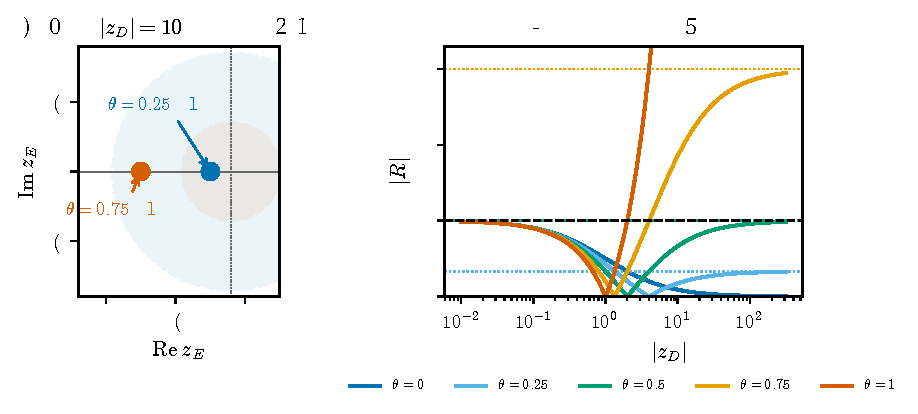
\includegraphics[width=0.96\textwidth]{stability_geometry.pdf}
  \caption{双变量稳定性函数的几何图像。(a) 固定 $|z_D|=10$ 时的稳定域圆盘与刚性射线上的点；(b) 沿刚性射线的放大因子，虚线为极限 $\theta/(1-\theta)$。}
  \label{fig:stability-geometry}
\end{figure}

图 \ref{fig:stability-region} 进一步给出了 $(\theta,\log_{10}|z_D|)$ 平面上的精确稳定域。黑色实线为 $|R|=1$ 的边界，其方程由 \eqref{eq:finite-threshold} 给出：
\begin{equation}
  \log_{10}|z_D|=\log_{10}\frac{2}{2\theta-1},\qquad \theta>\frac12.
  \label{eq:boundary-curve}
\end{equation}
$\theta\le1/2$ 的整个左半区域都是稳定的；$\theta>1/2$ 时，稳定域位于边界曲线下方。随着 $|z_D|$ 增大，允许的 $\theta$ 越来越接近 $1/2$。这张图可以看作分裂族的“相图”：它把稳定性问题转化为一个二维区域问题，便于设计参数。

\begin{figure}[htbp]
  \centering
  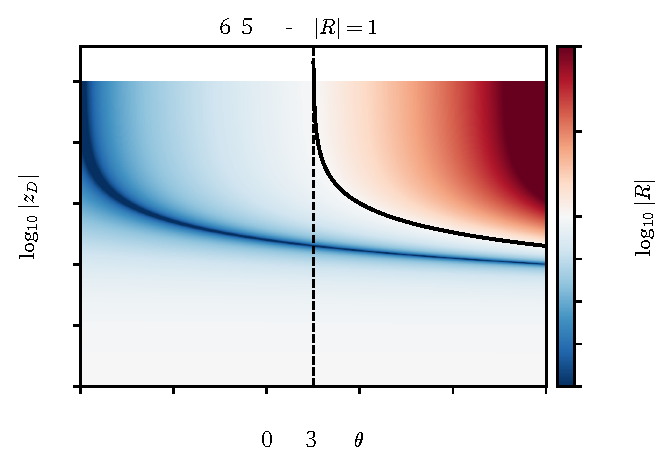
\includegraphics[width=0.72\textwidth]{stability_region.pdf}
  \caption{精确稳定域 $|R(z_E,z_I)|\le1$ 在 $(\theta,\log_{10}|z_D|)$ 平面上的相图。黑色实线为边界 \eqref{eq:boundary-curve}。}
  \label{fig:stability-region}
\end{figure}

\subsection{刚性极限}

由 \eqref{eq:R-ray}，当 $\theta<1$ 且 $x\to\infty$ 时
\begin{equation}
  \lim_{x\to\infty}R\left(-\theta x,-(1-\theta)x\right)
  =-\frac{\theta}{1-\theta}.
  \label{eq:R-infinity}
\end{equation}
其模为 $\theta/(1-\theta)$。条件 $|R_\infty|\le1$ 等价于 $\theta\le1/2$，与定理 \ref{thm:main} 一致。这个极限值有清晰的物理意义：在扩散主导的刚性极限下，显式部分把比例为 $\theta$ 的耗散“漏”了出去，隐式部分只能压住剩下的 $1-\theta$；两者之比决定了残余放大因子的幅度。

对 $\theta=1/2$，$R_\infty=-1$。这不是真正的衰减，而是每个时间步改变符号、幅度不变的寄生振荡。它在数值解中表现为网格尺度的锯齿波，虽然不发散，但会污染解的精度。这一点将在第五章的数值实验中得到验证。

\section{耦合刚性比与联合稳定域}
\label{sec:coupled-ratio}

\subsection{连续符号的联合稳定条件}

前面的定理只考虑了纯耗散情形 $\lambda_C=0$。实际计算中对流与扩散同时存在，因此需要把 $z_E$ 的实部（耗散）与虚部（对流）一起保留。对连续符号
\begin{equation}
  \lambda_C=-\ii ak,\qquad \lambda_D=-k^2,
\end{equation}
令
\begin{equation}
  \mu=ak\Delta t,\qquad d=\nu k^2\Delta t\ge0.
  \label{eq:mu-d}
\end{equation}
则
\begin{equation}
  z_E=-\ii\mu-\theta d,\qquad z_I=-(1-\theta)d.
  \label{eq:zE-continuous}
\end{equation}
代入 \eqref{eq:R-general} 得
\begin{equation}
  R=\frac{1-\theta d-\ii\mu}{1+(1-\theta)d}.
  \label{eq:R-continuous}
\end{equation}
稳定性条件 $|R|\le1$ 等价于
\begin{equation}
  (1-\theta d)^2+\mu^2\le\left(1+(1-\theta)d\right)^2.
  \label{eq:continuous-ineq}
\end{equation}
展开并整理，得到本文的第二个核心结论：
\begin{equation}
  \boxed{\ \mu^2\le 2d+(1-2\theta)d^2\ }.
  \label{eq:coupled-condition}
\end{equation}
当 $\mu=0$ 时，\eqref{eq:coupled-condition} 化为 $d[(1-2\theta)d+2]\ge0$，即定理 \ref{thm:main} 中的 $(1-2\theta)d+2\ge0$。因此，纯耗散定理是联合稳定条件在 $\mu=0$ 处的切片。

对固定的 $\theta$ 与 $d$，允许的对流强度为
\begin{equation}
  |\mu|\le\mu_{\max}(d)
  =\sqrt{\max\left\{0,\ 2d+(1-2\theta)d^2\right\}}.
  \label{eq:mu-max}
\end{equation}
当 $\theta\le1/2$ 时，根号内的二次式对一切 $d\ge0$ 非负，稳定域向 $d$ 方向无限延伸；当 $\theta>1/2$ 时，二次式在
\begin{equation}
  d>d_c=\frac{2}{2\theta-1}
  \label{eq:dc}
\end{equation}
时变负，此时即使 $\mu=0$ 也不稳定，这与定理 \ref{thm:main} 的有限阈值完全一致。

在长波极限 $d\to0$ 下，$\mu_{\max}\approx\sqrt{2d}$，与 $\theta$ 无关；在 $d\to\infty$ 时，
\begin{equation}
  \mu_{\max}\sim
  \begin{cases}
    \sqrt{1-2\theta}\,d, & \theta<1/2,\\[4pt]
    \sqrt{2d}, & \theta=1/2.
  \end{cases}
  \label{eq:mu-asymptotic}
\end{equation}
这说明：当隐式部分至少承担一半耗散时，对流可以按 $O(d)$ 的速度增长而不破坏稳定性；当 $\theta=1/2$ 时，对流的容许量只按 $\sqrt d$ 增长；当 $\theta>1/2$ 时，稳定域在 $d_c$ 处终止。

\subsection{耦合刚性比与 \texorpdfstring{$\beta_\infty(\varepsilon)$}{beta-inf}}

联合稳定条件还可以用“刚性比”的语言表述。设 $z_E$ 与 $z_I$ 按固定比例同时趋于无穷：
\begin{equation}
  z_I=\varepsilon z_E,\qquad |z_E|\to\infty,\qquad \varepsilon\ne0.
  \label{eq:epsilon-def}
\end{equation}
则
\begin{equation}
  R=\frac{1+z_E}{1-\varepsilon z_E}
  \longrightarrow
  \beta_\infty(\varepsilon)=-\frac{1}{\varepsilon}.
  \label{eq:beta-infinity}
\end{equation}
称 $\beta_\infty(\varepsilon)$ 为耦合刚性极限的放大因子。格式在该极限下稳定，当且仅当
\begin{equation}
  |\beta_\infty(\varepsilon)|\le1
  \iff
  |\varepsilon|\ge1.
  \label{eq:epsilon-stable}
\end{equation}
对本文的 $\theta$ 族，沿纯耗散射线有
\begin{equation}
  \varepsilon=\frac{z_I}{z_E}=\frac{1-\theta}{\theta},
  \qquad \theta\in(0,1].
  \label{eq:epsilon-theta}
\end{equation}
于是
\begin{equation}
  |\varepsilon|\ge1
  \iff
  \frac{1-\theta}{\theta}\ge1
  \iff
  \theta\le\frac12,
  \label{eq:epsilon-half}
\end{equation}
与 \eqref{eq:theta-half} 完全一致。这个推导把“显式与隐式各承担多少”翻译成一个无量纲比值：$\varepsilon$ 越大，隐式部分相对越强；$\varepsilon=1$ 是临界点，$\varepsilon<1$ 时显式部分过强，刚性极限下的残余放大因子的模超过 $1$。当 $\theta=1$ 时 $\varepsilon=0$，没有隐式部分，$R=1+z_E$ 无界，不属于上述极限。

需要强调，$\beta_\infty(\varepsilon)$ 是 IMEX-Euler 的普适函数，与具体的空间算子无关；分裂族只负责在曲线 $\varepsilon=(1-\theta)/\theta$ 上选点。这一观点把“设计分裂”转化为“在 $|\beta_\infty(\varepsilon)|\le1$ 的区域内选 $\varepsilon$”，比逐点检查 $|R|$ 更便于推广到其他格式。

\subsection{几何图像}

图 \ref{fig:stability-coupled}(a) 画出了 $\mu_{\max}(d)$ 随 $d$ 的变化。曲线下方为稳定区，上方为不稳定区；$\theta>1/2$ 的曲线在 $d_c$ 处终止。图 \ref{fig:stability-coupled}(b) 画出了 $|\beta_\infty(\varepsilon)|=1/|\varepsilon|$，并标出了 $|\varepsilon|\ge1$ 的稳定侧。两张图从不同角度描述同一件事：稳定性由“显式部分与隐式部分的相对强度”决定，而不是由某一个单独的稳定性参数决定。

\begin{figure}[htbp]
  \centering
  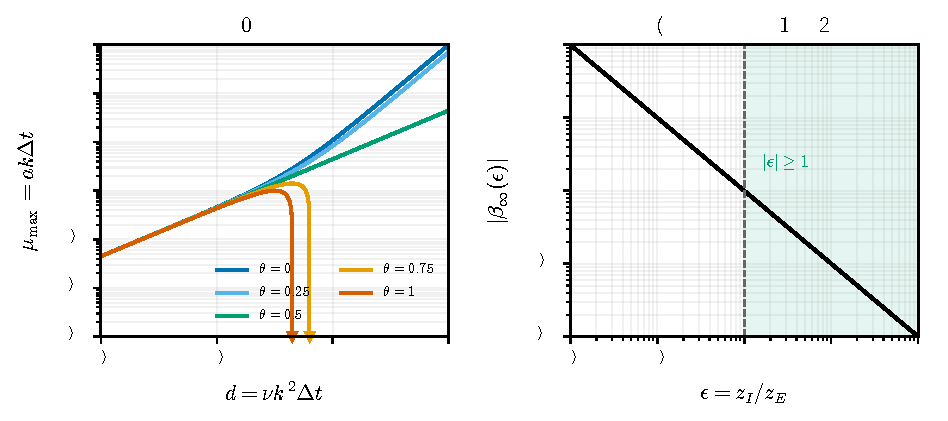
\includegraphics[width=0.96\textwidth]{stability_coupled.pdf}
  \caption{连续符号下的联合稳定域。(a) 曲线 $\mu_{\max}(d)$ 下方为稳定区；$\theta>1/2$ 时曲线在 $d=2/(2\theta-1)$ 处终止。(b) 刚性极限放大因子 $|\beta_\infty(\varepsilon)|=1/|\varepsilon|$；$|\varepsilon|\ge1$ 时不超过 $1$。}
  \label{fig:stability-coupled}
\end{figure}

图 \ref{fig:stability-coupled}(a) 还揭示了两种不同的失稳机制。第一种是“耗散不足”：当 $\theta>1/2$ 且 $d>d_c$ 时，隐式部分压不住显式耗散，纯耗散模态本身就不稳定；第二种是“对流—扩散失衡”：当 $d$ 较小而 $\mu$ 较大时，显式对流项超出圆盘所能容纳的范围。前者由 $\theta$ 控制，后者由 $\mu/d$ 控制。第 \ref{sec:discrete-symbol} 节将说明，离散格式的网格尺度失稳属于第一种机制，而长波失稳属于第二种机制。

\section{L-稳定与刚性衰减}
\label{sec:L-stability}

\begin{table}[htbp]
  \centering
  \small
  \setlength{\tabcolsep}{5pt}
  \caption{不同 $\theta$ 的稳定性性质}
  \label{tab:theta-stability}
  \begin{tabular}{lcccc}
    \toprule
    $\theta$ & $R_\infty$ & 刚性稳定 & L-稳定 & 表现 \\
    \midrule
    $0$ & $0$ & 所有 $x$ & 是 & 强阻尼 \\
    $(0,\frac12)$ & $-\frac{\theta}{1-\theta}$ & 所有 $x$ & 否 & 有界振荡 \\
    $\frac12$ & $-1$ & 所有 $x$ & 否 & 临界振荡 \\
    $(\frac12,1)$ & $|R_\infty|>1$ & $x\le\frac{2}{2\theta-1}$ & 否 & 大 $x$ 失稳 \\
    $1$ & $-\infty$ & $x\le2$ & 否 & 条件稳定 \\
    \bottomrule
  \end{tabular}
\end{table}

表 \ref{tab:theta-stability} 汇总了各种情形的稳定性。可以得到如下结论。

第一，只有 $\theta=0$ 是沿刚性射线 L-稳定的。此时 $R=1/(1+x)\to0$，最快的耗散模态被完全压掉。这与经典理论中“全隐式 Euler 是 L-稳定的”一致。

第二，$0<\theta\le1/2$ 沿刚性射线稳定，但不是 L-稳定的。其极限放大因子为 $-\theta/(1-\theta)$，绝对值小于 $1$（$\theta=1/2$ 时等于 $1$）。这意味着格式不会发散，但也不会把刚性模态完全衰减；在长时间计算中，这些模态可能以低频振荡的形式残留。

第三，$\theta=1/2$ 是临界情形。它恰好满足 $|R_\infty|=1$，属于“中性稳定”。它没有稳定裕度；在非线性计算中，若同时存在其他失稳机制（例如边界反射、限制器开关），可能表现为网格尺度的弱振荡。因此，在实际计算中不宜把 $\theta=1/2$ 当作安全边界：它是理论上的分界点，而不是工程上的推荐值。

第四，$\theta>1/2$ 只在一个有限的刚性范围内稳定。随着网格加密或 $\nu$ 增大，$|z_D|$ 增大，格式终将失稳。这一结论对时间步长控制有直接影响：不能简单地用 CFL 条件来选取 $\Delta t$，还必须考虑扩散刚性。

\section{离散符号与 CFL 条件}
\label{sec:discrete-symbol}

定理 \ref{thm:main} 与联合条件 \eqref{eq:coupled-condition} 是对连续符号的结论。实际计算使用的是全离散格式，其稳定性由 \eqref{eq:symbols} 的离散符号决定。本节给出离散情形的分析，并说明它与连续结论的关系。

\subsection{全离散放大因子}

将 \eqref{eq:symbols} 代入 \eqref{eq:zE-zI}，记
\begin{equation}
  c=\frac{a\Delta t}{\Delta x},\qquad
  r=\frac{\nu\Delta t}{\Delta x^2},\qquad
  q=1-\cos\xi\in[0,2],
  \label{eq:c-r-q}
\end{equation}
并令
\begin{equation}
  \delta=cq,\qquad \mu=c\sin\xi,\qquad d=2rq.
  \label{eq:delta-mu-d}
\end{equation}
则
\begin{equation}
  z_E=-\delta-\theta d-\ii\mu,
  \qquad
  z_I=-(1-\theta)d,
  \label{eq:zE-discrete}
\end{equation}
放大因子为
\begin{equation}
  R(\xi)=\frac{1-\delta-\theta d-\ii\mu}{1+(1-\theta)d}.
  \label{eq:R-discrete}
\end{equation}
稳定性条件 $|R(\xi)|\le1$ 对任意 $\xi\in[0,\pi]$ 成立。直接对 $\xi$ 扫描即可得到数值稳定域；下面给出两个有解析表达的极端情形。

\subsection{网格尺度分析}

在网格尺度 $\xi=\pi$ 处，$q=2$，$\delta=2c$，$\mu=0$，$d=4r$。代入 \eqref{eq:R-discrete} 得
\begin{equation}
  z_E=-2c-4\theta r,\qquad z_I=-4(1-\theta)r,
  \label{eq:sawtooth}
\end{equation}
稳定性条件为
\begin{equation}
  \left|1-2c-4\theta r\right|\le1+4(1-\theta)r.
  \label{eq:sawtooth-ineq}
\end{equation}
对 $\theta>1/2$ 且 $r$ 较大，左端为 $2c+4\theta r-1$，右端为 $1+4(1-\theta)r$，于是
\begin{equation}
  2c+4(2\theta-1)r\le2
  \iff
  c+2(2\theta-1)r\le1.
  \label{eq:sawtooth-condition}
\end{equation}
这就是 $\theta>1/2$ 时的扩散限制。几个特例如下：
\begin{align}
  \theta=1:&\qquad c+2r\le1; \label{eq:theta1-cfl}\\
  \theta=3/4:&\qquad c+r\le1; \label{eq:theta34-cfl}\\
  \theta=1/2:&\qquad c\le1. \label{eq:theta12-cfl}
\end{align}
当 $c$ 很小时（扩散主导），\eqref{eq:theta1-cfl} 给出 $r\le1/2$，即 $\Delta t\le\Delta x^2/(2\nu)$，这正是显式扩散的标准稳定性条件。对 $\theta=3/4$，条件放宽为 $r\le1$；对 $\theta=1/2$，扩散限制消失，只剩下 CFL 条件 $c\le1$。

\subsection{长波分析与数值耗散}

对 $\theta\le1/2$，网格尺度是稳定的（$\theta<1/2$）或退化为 $c\le1$（$\theta=1/2$），此时限制可能来自长波。把 \eqref{eq:symbols-long-wave} 代入连续稳定性条件，等价地，在 \eqref{eq:R-discrete} 中令 $\xi\to0$。由
\begin{equation}
  \delta\approx\frac{c}{2}\xi^2,\qquad
  d\approx r\xi^2,\qquad
  \mu\approx c\xi,
\end{equation}
并只保留 $\xi^2$ 阶项，\eqref{eq:R-discrete} 的稳定性条件给出
\begin{equation}
  c^2\le c+2r.
  \label{eq:long-wave-c-r}
\end{equation}
把 $c=a\Delta t/\Delta x$、$r=\nu\Delta t/\Delta x^2$ 代入，整理得
\begin{equation}
  \Delta t\le\frac{2\nu+|a|\Delta x}{a^2}.
  \label{eq:low-k-numerical}
\end{equation}
若忽略 Rusanov 的数值耗散（即把 $|a|\Delta x$ 项去掉），则回到
\begin{equation}
  \Delta t\le\frac{2\nu}{a^2}.
  \label{eq:low-k-condition}
\end{equation}
注意这个条件与 $\Delta x$ 无关，它是一个“扩散时间尺度”条件，而不是 CFL 条件。当 $\nu$ 较大时，它允许较大的 $\Delta t$；当 $\nu$ 较小时，它变得严格。

条件 \eqref{eq:long-wave-c-r} 有一个重要的推论：当 $\theta<1/2$ 时，隐式扩散足够强，CFL 数可以远大于 $1$。例如取 $\nu=1$、$a=1$、$\Delta x=0.005$，\eqref{eq:low-k-numerical} 给出 $\Delta t\lesssim2.005$，对应的 $c\approx401$。这解释了第五章中 $\theta=0$ 与 $\theta=1/4$ 的最大步长约为 $2.05$ 的现象：限制来自扩散时间尺度，而不是对流 CFL 条件。对 $\theta=1/2$，网格尺度条件 \eqref{eq:theta12-cfl} 给出 $\Delta t\le\Delta x/a$，它比 \eqref{eq:low-k-numerical} 更严格，因此最大步长在 $\theta=1/2$ 处出现断崖式下降。

图 \ref{fig:stability-discrete} 给出了固定 $\CFL=0.4$、$\nu=1$、$N=200$ 时 $|R(\xi)|$ 随 $\xi$ 的变化。此时 $\nu\Delta t/\Delta x^2=80$，属于强扩散情形。$\theta=0$、$0.25$、$0.5$ 的曲线始终不超过 $1$；$\theta=0.6$、$0.75$、$1$ 的曲线在某个波数之后穿过 $1$，并迅速上升（$\theta=1$ 更早，因为全部耗散都在显式部分）。这正是 $\theta>1/2$ 时网格尺度失稳的直接证据，也是 \eqref{eq:sawtooth-condition} 中 $r$ 项占主导的体现。

\begin{figure}[htbp]
  \centering
  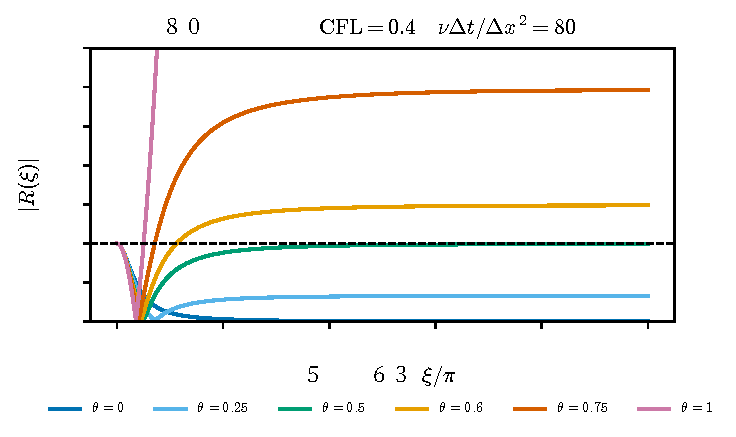
\includegraphics[width=0.78\textwidth]{stability_discrete.pdf}
  \caption{全离散放大因子 $|R(\xi)|$ 随无量纲波数的变化（$\CFL=0.4$，$\nu\Delta t/\Delta x^2=80$）。虚线为 $|R|=1$。}
  \label{fig:stability-discrete}
\end{figure}

\subsection{离散稳定性的完整图像}

综合以上分析，离散格式的稳定性可以概括为：

\begin{enumerate}[label=(\roman*),leftmargin=2.4em]
  \item 当 $\theta<1/2$ 时，网格尺度无条件稳定；时间步长由长波条件 \eqref{eq:low-k-numerical} 控制。此时 CFL 数可以大于 $1$，甚至远大于 $1$，但格式的精度会下降。
  \item 当 $\theta=1/2$ 时，网格尺度条件退化为 $c\le1$，长波条件仍为 \eqref{eq:low-k-numerical}；最大步长由两者中较小者决定。对本文的参数（$\nu=1$，$N=200$），$c\le1$ 是起决定作用的约束，因此 $\Delta t_{\max}=\Delta x$。
  \item 当 $\theta>1/2$ 时，除长波条件外，还必须满足网格尺度条件 \eqref{eq:sawtooth-condition}。随着 $\theta\to1$，该条件趋于 $c+2r\le1$，即显式扩散的经典限制。
  \item 无论 $\theta$ 取何值，$\Delta t$ 都不能由单一的 CFL 条件确定；必须同时检查 $c$、$r$ 与刚性参数 $z_D$。
\end{enumerate}

\section{讨论}
\label{sec:discussion}

\subsection{为什么边界是 \texorpdfstring{$1/2$}{1/2}}

定理 \ref{thm:main} 的证明只用了初等代数，但 $1/2$ 的出现并非偶然。在刚性射线上，显式部分承担的耗散比例为 $\theta$，隐式部分为 $1-\theta$。当 $x\to\infty$ 时，显式部分的放大因子为 $-\theta x$，隐式部分的分母为 $(1-\theta)x$。两者之比为 $-\theta/(1-\theta)$。要求其模不超过 $1$，自然得到 $\theta\le1/2$。从几何上看，这是射线斜率 $\theta$ 与圆盘半径斜率 $1-\theta$ 的竞争。因此，$1/2$ 是“显式与隐式各承担一半”的临界点，具有明确的物理意义。

\subsection{与 Zakerzadeh--Noelle 判据的关系}

Zakerzadeh 与 Noelle 在研究刚性双曲守恒律的 IMEX 通量分裂时，系统比较了对称分裂与非对称分裂：对称分裂可以做到对刚性参数一致稳定，而非对称分裂不一定；他们通过具体算例说明，某些看似自然的分裂会出现小范围的不稳定\cite{zakerzadeh2018}。用本文的语言，这说明“把刚性项放进隐式部分”只是容许性的必要条件，而不是充分条件；分裂的对称性与结构同样重要。本文的 $\theta$ 族是非对称分裂，因此需要逐点分析；定理 \ref{thm:main} 给出的 $\theta\le1/2$ 正是这种分析的结果。与他们的判据相比，本文的结论更细：$\theta\le1/2$ 虽然不是 L-稳定的，但沿刚性射线仍然是稳定的；它在有限刚性下可用，只是在极强的刚性下会留下不衰减的残余模态。

\subsection{线性分析的局限}

本章的分析基于线性化与冻结系数。对非线性 Burgers 方程，激波附近的系数变化、限制器的开关、边界条件等都可能影响稳定性。线性分析给出的是必要条件：如果线性化格式不稳定，非线性格式必然不稳定；反之，线性稳定并不保证非线性稳定。因此，第五章的数值实验不仅是对理论的验证，也是对非线性效应的补充。实验中采用的 MUSCL/minmod 重构具有 TVD 性质，可以在一定程度上抑制非线性振荡；但限制器在极值点附近退化为一阶，也会影响精度。这些因素在解读实验结果时都需要考虑。

\subsection{稳定性与精度的张力}

从表 \ref{tab:theta-stability} 可以看到，$\theta=0$ 具有最好的稳定性，但它的隐式部分最“重”；$\theta=1/2$ 的计算最便宜（隐式部分只有一半），但处于临界状态。稳定性与精度并不是同一个问题：一个格式可以稳定但过度耗散，也可以精确但脆弱。第五章将用激波算例说明，在稳定的前提下，$\theta$ 对精度的影响是温和的；真正决定精度的是空间格式的阶数与数值耗散，而不是 $\theta$ 本身。

\section{本章小结}

本章建立了参数化分裂族的稳定性理论。主要结果包括：
\begin{enumerate}[label=(\arabic*),leftmargin=2.4em]
  \item 双变量稳定性函数 $R(z_E,z_I)=(1+z_E)/(1-z_I)$ 及其圆盘表示；
  \item 纯耗散情形下的精确条件 $(1-2\theta)x+2\ge0$，即 $\theta\le1/2$ 时对所有刚性稳定，$\theta>1/2$ 时仅对 $x\le2/(2\theta-1)$ 稳定；
  \item 连续符号下的联合稳定条件 $\mu^2\le2d+(1-2\theta)d^2$，以及刚性比表述 $|\beta_\infty(\varepsilon)|=1/|\varepsilon|$，$|\varepsilon|\ge1$；
  \item 只有 $\theta=0$ 沿刚性射线 L-稳定，$\theta=1/2$ 是临界稳定；
  \item 全离散符号分析给出了 $\theta>1/2$ 时的网格尺度条件 $c+2(2\theta-1)r\le1$，以及长波条件 $\Delta t\le(2\nu+|a|\Delta x)/a^2$。
\end{enumerate}
这些结果为第五章的数值验证提供了明确的可检验预测。

% ==========================================================================
\chapter{数值验证}
% ==========================================================================

本章用数值实验检验第四章的理论预测。第 \ref{sec:exp-design} 节说明实验设计与误差度量；第 \ref{sec:stiff-map} 节给出刚性相图；第 \ref{sec:max-dt} 节比较最大稳定步长；第 \ref{sec:shock-accuracy} 节定量分析激波精度；第 \ref{sec:convergence} 节验证网格收敛性；第 \ref{sec:exp-discussion} 节讨论稳定性与精度的关系。

\section{实验设计}
\label{sec:exp-design}

所有实验均基于第三章的有限体积半离散格式与 IMEX-Euler 时间推进。代码以 Python 实现，空间算子采用一阶 Rusanov 通量（稳定性实验）或 MUSCL/minmod 重构（精度实验），时间推进使用固定步长的 IMEX-Euler。线性系统用稀疏 LU 分解求解，矩阵在步长固定时只分解一次。

实验分为四组，分别回答四个问题：
\begin{enumerate}[label=(\arabic*),leftmargin=2.4em]
  \item 固定 CFL、扫描 $\nu$ 与 $\theta$，稳定性区域是否与 $\theta\le1/2$ 的预测一致？
  \item 固定 $\nu$、扫描 $\theta$，最大稳定步长如何随 $\theta$ 变化？是否与定理 \ref{thm:main} 及离散条件 \eqref{eq:sawtooth-condition} 一致？
  \item 在稳定的参数下，不同 $\theta$ 对激波位置、过渡层厚度和 $L^1$ 误差有何影响？
  \item 空间网格加密时，格式的观测收敛阶是多少？
\end{enumerate}

误差度量定义如下。设数值解为 $u_j$，精确解为 $u_{\rm ex}(x_j,t)$，定义平均 $L^1$ 误差
\begin{equation}
  E_1=\frac{1}{|\Omega|}\int_\Omega|u-u_{\rm ex}|\,\dd x,
  \label{eq:L1-error}
\end{equation}
用梯形公式计算。激波位置 $x_s$ 定义为 $u=0.5$ 的等值点，用线性插值确定；过渡层厚度 $w$ 定义为 $u=0.9$ 与 $u=0.1$ 两个等值点之间的距离。精确解的对应量为 $x_s^{\rm ex}=st$ 与 $w_{\rm ex}=4\nu\ln9/A$。

稳定性判据采用两种方式。对线性分析，直接计算所有 Fourier 模态的放大因子，若 $\max_\xi|R(\xi)|\le1$ 则判定稳定。对稳定性实验中的非线性计算，若解的最大模超过 $0.55$（约为初始最大模 $0.5$ 的 $1.1$ 倍）或出现非有限值，则判定失稳。

\section{刚性相图}
\label{sec:stiff-map}

第一组实验固定 $N=200$、$\Delta t=0.4\Delta x$、$t=1$，在周期区间 $[0,1]$ 上取初始条件
\begin{equation}
  u_0(x)=0.5+0.01\sin(2\pi x),
  \label{eq:smooth-ic}
\end{equation}
扫描 $\nu\in[10^{-2},10^{2}]$（对数网格，21 个点）与 $\theta\in[0,1]$（41 个点），记录终时刻的 $\max|u|$。稳定时 $\max|u|\approx0.5$；失稳时该值迅速增大。结果画成 $(\theta,\log_{10}\nu)$ 平面上的热图，颜色表示 $\log_{10}\max|u|$。

\begin{figure}[htbp]
  \centering
  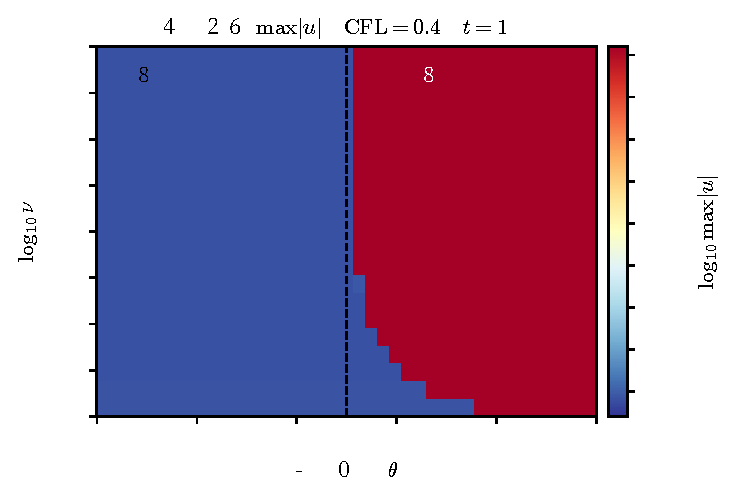
\includegraphics[width=0.74\textwidth]{stiff_heatmap.pdf}
  \caption{刚性相图：固定 $\CFL=0.4$、$N=200$、$t=1$，扫描 $\theta$ 与 $\nu$。颜色为 $\log_{10}\max|u|$；虚线为 $\theta=1/2$。}
  \label{fig:stiff-map}
\end{figure}

图 \ref{fig:stiff-map} 显示了一个清晰的相变：$\theta\le1/2$ 的整个左半区域保持稳定（深蓝色），$\theta>1/2$ 的区域在 $\nu$ 较大时变为红色（失稳）。分界线与 $\theta=1/2$ 的竖直虚线高度吻合。具体而言：

\begin{itemize}[leftmargin=2.2em]
  \item $\theta=0$、$0.25$、$0.5$ 在所有测试的 $\nu$ 下都稳定，包括 $\nu=100$ 的强刚性情形；
  \item $\theta=0.55$ 时，$\nu\lesssim0.06$ 稳定，$\nu\gtrsim0.1$ 失稳；
  \item $\theta=0.6$ 时，阈值约为 $\nu\approx0.03$；
  \item $\theta=0.75$ 时，阈值约为 $\nu\approx0.0125$；
  \item $\theta=1$ 时，即使 $\nu=0.01$ 也已失稳，因为此时 $r=\nu\Delta t/\Delta x^2=0.8>1/2$，显式扩散本身就不稳定。
\end{itemize}

这些阈值可以用网格尺度条件 \eqref{eq:sawtooth-condition} 定量解释。在 $\xi=\pi$ 处，$c=\Delta t/\Delta x=0.4$，$r=\nu\Delta t/\Delta x^2=80\nu$（取 $\Delta x=0.005$）。由 $c+2(2\theta-1)r\le1$ 解出
\begin{equation}
  \nu\le\nu_{\max}=\frac{\Delta x^2}{2\Delta t(2\theta-1)}
  =\frac{6.25\times10^{-3}}{2\theta-1}.
  \label{eq:nu-max}
\end{equation}
对 $\theta=0.55$、$0.6$、$0.75$、$1$，分别得到 $\nu_{\max}=0.0625$、$0.03125$、$0.0125$、$0.00625$，与热图中的转变位置一致。这说明相图的边界不是数值偶然，而是由离散符号精确决定的。

\section{最大稳定步长}
\label{sec:max-dt}

第二组实验固定 $N=200$、$\nu=1$，在周期区间上取初始条件 \eqref{eq:smooth-ic}，并叠加一个幅度为 $10^{-8}$ 的网格尺度扰动 $(-1)^j$。这个种子是必要的：若初值完全光滑，网格尺度模态不会被激发，有限时间的二分法会高估稳定步长。对每个 $\theta$，用二分法寻找最大的稳定步长；每次试验固定推进 $20000$ 步，而不是固定物理终时，因为稳定性是每步性质。

线性预测通过扫描所有 $\xi\in[0,\pi]$、要求 $\max|R(\xi)|\le1$ 得到。图 \ref{fig:max-dt} 给出了 $\Delta t_{\max}$ 随 $\theta$ 的变化（对数纵轴）。曲线呈现出两个截然不同的区域：

\begin{figure}[htbp]
  \centering
  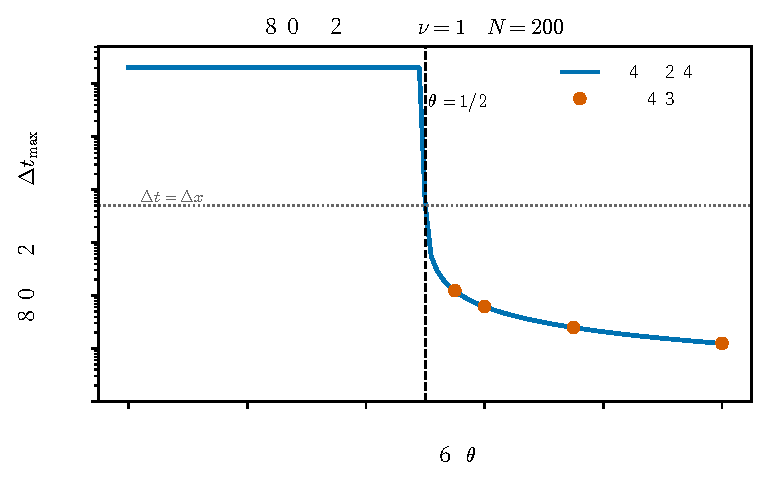
\includegraphics[width=0.74\textwidth]{maxdt.pdf}
  \caption{最大稳定步长随 $\theta$ 的变化（$\nu=1$，$N=200$，$\Delta x=0.005$）。实线为线性稳定性预测，圆点为非线性实验；虚线为 $\theta=1/2$。}
  \label{fig:max-dt}
\end{figure}

\begin{itemize}[leftmargin=2.2em]
  \item 当 $\theta<1/2$ 时，$\Delta t_{\max}$ 几乎不变，约为 $2.05$。此时稳定性由低波数扩散条件 \eqref{eq:low-k-numerical} 控制，而不是 CFL 条件。代入 $\nu=1$、$\Delta x=0.005$、$a=1$，得 $(2\nu+\Delta x)/a^2=2.005$，线性符号预测为 $2.056$，略高于渐近值，这是离散符号的修正。
  \item 当 $\theta=1/2$ 时，$\Delta t_{\max}$ 突然降到 $\Delta x=0.005$。此时网格尺度条件退化为 $c\le1$，即 $\Delta t\le\Delta x$；低波数条件虽然允许更大的步长，但 $c\le1$ 成为起决定作用的约束。
  \item 当 $\theta>1/2$ 时，$\Delta t_{\max}$ 按 $1/(2\theta-1)$ 衰减。由 \eqref{eq:sawtooth-condition} 得
  \begin{equation}
    \Delta t_{\max}=\frac{\Delta x^2}{2\nu(2\theta-1)}.
    \label{eq:dt-max-formula}
  \end{equation}
  对 $\theta=0.55,0.6,0.75,1$，实测值与线性符号预测分别相差 $1.6\%$、$0.8\%$、$0.3\%$、$0.2\%$；与渐近公式 \eqref{eq:dt-max-formula} 的差别更小。
\end{itemize}

表 \ref{tab:max-dt} 汇总了代表性结果。需要强调，$\theta=1/2$ 的“突然下降”并不是说格式在 $\theta=1/2$ 处不稳定；它仍然稳定，只是允许的步长从“扩散控制”切换到了“CFL 控制”。这一切换是最大步长曲线出现断崖的原因。

\begin{table}[htbp]
  \centering
  \caption{不同 $\theta$ 下的最大稳定步长（$\nu=1$，$N=200$，$\Delta x=0.005$）}
  \label{tab:max-dt}
  \begin{tabular}{ccccc}
    \toprule
    $\theta$ & 理论公式 \eqref{eq:dt-max-formula} & 线性符号预测 & 非线性实验 & 相对偏差 \\
    \midrule
    $0$     & 无（扩散控制） & $2.056$ & --- & --- \\
    $0.25$  & 无（扩散控制） & $2.030$ & --- & --- \\
    $0.5$   & $\Delta x=5.000\times10^{-3}$ & $5.000\times10^{-3}$ & --- & --- \\
    $0.55$  & $1.250\times10^{-4}$ & $1.220\times10^{-4}$ & $1.239\times10^{-4}$ & $1.6\%$ \\
    $0.6$   & $6.250\times10^{-5}$ & $6.173\times10^{-5}$ & $6.223\times10^{-5}$ & $0.8\%$ \\
    $0.75$  & $2.500\times10^{-5}$ & $2.488\times10^{-5}$ & $2.496\times10^{-5}$ & $0.3\%$ \\
    $1$     & $1.250\times10^{-5}$ & $1.247\times10^{-5}$ & $1.249\times10^{-5}$ & $0.2\%$ \\
    \bottomrule
  \end{tabular}
\end{table}

表中“相对偏差”以线性符号预测为基准。对 $\theta<1/2$，线性阈值来自长波条件 \eqref{eq:low-k-numerical}；在 $L=1$、$N=200$ 的周期域上，第一个离散波数 $k=2\pi$ 已经落在不稳定带之外，因此有限时间内观察不到失稳。对 $\theta=1/2$，最不稳定模态是网格尺度，但其增长率在临界点附近趋于零，$20000$ 步内不足以把 $10^{-8}$ 的种子放大到可测幅度。这两种情形的非线性实验记为“---”，以线性符号预测为准；$\theta\ge0.55$ 的实验点则与预测吻合到 $2\%$ 以内。

\section{激波精度}
\label{sec:shock-accuracy}

第三组实验在 $[-2,3]$ 上计算粘性激波，取 $\nu=0.01$、$u_L=1$、$u_R=0$、$t=2$，初始条件为精确解 \eqref{eq:exact-shock} 在 $t=0$ 的值。网格 $N=800$，$\Delta x=6.25\times10^{-3}$，$\CFL=0.2$。此时 $r=\nu\Delta t/\Delta x^2=0.32<1/2$，所有 $\theta$ 都稳定。分别用一阶 Rusanov 与 MUSCL/minmod 计算 $\theta=0,0.25,0.5,0.75,1$ 五组解。

\begin{figure}[htbp]
  \centering
  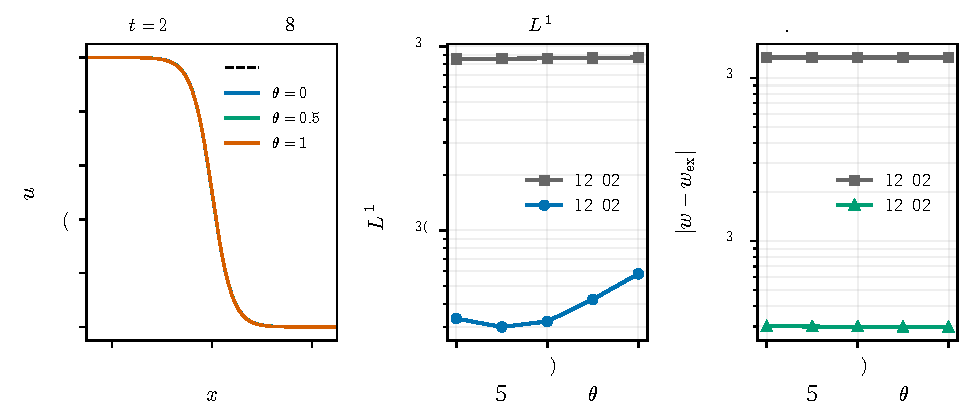
\includegraphics[width=0.98\textwidth]{shock_results.pdf}
  \caption{粘性激波的数值结果（$\nu=0.01$，$N=800$，$\CFL=0.2$，$t=2$）。(a) 剖面；(b) $L^1$ 误差随 $\theta$ 的变化；(c) 过渡层厚度误差随 $\theta$ 的变化。}
  \label{fig:shock-results}
\end{figure}

图 \ref{fig:shock-results}(a) 给出了 $\theta=0,0.5,1$ 的剖面与精确解。三条曲线在视觉上几乎重合，说明在稳定的参数下，$\theta$ 对整体波形的影响很小。差异体现在误差指标上。

\begin{table}[htbp]
  \centering
  \caption{激波算例的误差指标（$N=800$，$\nu=0.01$，$t=2$，$\CFL=0.2$）}
  \label{tab:shock-metrics}
  \small
  \begin{tabular}{ccccc}
    \toprule
    $\theta$ & \multicolumn{2}{c}{一阶 Rusanov} & \multicolumn{2}{c}{MUSCL/minmod} \\
    \cmidrule(lr){2-3}\cmidrule(lr){4-5}
     & $E_1$ & $|x_s-x_s^{\rm ex}|$ & $E_1$ & $|x_s-x_s^{\rm ex}|$ \\
    \midrule
    $0$    & $8.543\times10^{-4}$ & $1.395\times10^{-3}$ & $3.322\times10^{-5}$ & $1.041\times10^{-4}$ \\
    $0.25$ & $8.573\times10^{-4}$ & $1.477\times10^{-3}$ & $2.992\times10^{-5}$ & $8.40\times10^{-6}$ \\
    $0.5$  & $8.602\times10^{-4}$ & $1.560\times10^{-3}$ & $3.207\times10^{-5}$ & $8.73\times10^{-5}$ \\
    $0.75$ & $8.651\times10^{-4}$ & $1.642\times10^{-3}$ & $4.222\times10^{-5}$ & $1.831\times10^{-4}$ \\
    $1$    & $8.700\times10^{-4}$ & $1.725\times10^{-3}$ & $5.812\times10^{-5}$ & $2.788\times10^{-4}$ \\
    \bottomrule
  \end{tabular}
\end{table}

由表 \ref{tab:shock-metrics} 与图 \ref{fig:shock-results} 可以得到以下观察。

第一，一阶格式的误差主要由数值扩散主导。精确过渡层厚度为 $w_{\rm ex}=0.08789$，一阶格式给出 $w\approx0.10125$，相对误差约 $15.2\%$。这部分数值扩散来自 Rusanov 通量，其系数约为 $\Delta x/2=3.1\times10^{-3}$，远大于物理粘性 $\nu=0.01$ 的高波数贡献。不同 $\theta$ 的 $E_1$ 只相差约 $1.8\%$（从 $8.543\times10^{-4}$ 到 $8.700\times10^{-4}$），说明在一阶精度下，$\theta$ 的影响被空间误差掩盖。

第二，MUSCL 重构显著降低了误差。$E_1$ 从 $8.5\times10^{-4}$ 降到 $3.0\times10^{-5}$ 至 $5.8\times10^{-5}$，降低约 $15$ 至 $28$ 倍；过渡层厚度的误差从 $1.34\times10^{-2}$ 降到 $3.0\times10^{-4}$，降低约 $45$ 倍。这说明空间重构是提高精度的主要途径。

第三，在 MUSCL 格式中，$\theta$ 的影响变得可见，但不是单调的。$\theta=0.25$ 给出最小的 $E_1=2.992\times10^{-5}$ 与最小的位置误差 $8.4\times10^{-6}$；$\theta=0.5$ 次之（$3.207\times10^{-5}$），$\theta=0$ 第三（$3.322\times10^{-5}$）；$\theta=1$ 给出最大的 $E_1=5.812\times10^{-5}$，约为最优值的 $1.94$ 倍。这与“隐式越多越耗散”的直觉部分一致：$\theta=0$ 的隐式扩散最强，会增加一点数值耗散；$\theta=1$ 的显式扩散最弱，但会在激波附近留下轻微的振荡（$L^\infty$ 误差从 $2.50\times10^{-3}$ 增至 $4.34\times10^{-3}$）。$\theta=0.25$ 在两者之间取得了平衡。

第四，所有 $\theta$ 在 $\CFL=0.2$ 下都是稳定的，但稳定性边界并不相同。若把 $\CFL$ 提高到 $0.4$，$\theta=0.75$ 与 $1$ 会失稳（因为 $r=0.64>1/2$ 且 $c+r>1$），而 $\theta\le0.5$ 仍然稳定。因此，“哪个 $\theta$ 更准确”的比较必须在共同的稳定区域内进行；离开稳定区域，精度无从谈起。

\section{网格收敛性}
\label{sec:convergence}

第四组实验固定 $\nu=0.01$、$\CFL=0.2$、$t=1$，取 $N=100,200,400,800$，分别计算一阶格式（$\theta=0.5$）与 MUSCL 格式（$\theta=0,0.5$）的 $L^1$ 误差。结果如图 \ref{fig:convergence} 与表 \ref{tab:convergence} 所示。

\begin{figure}[htbp]
  \centering
  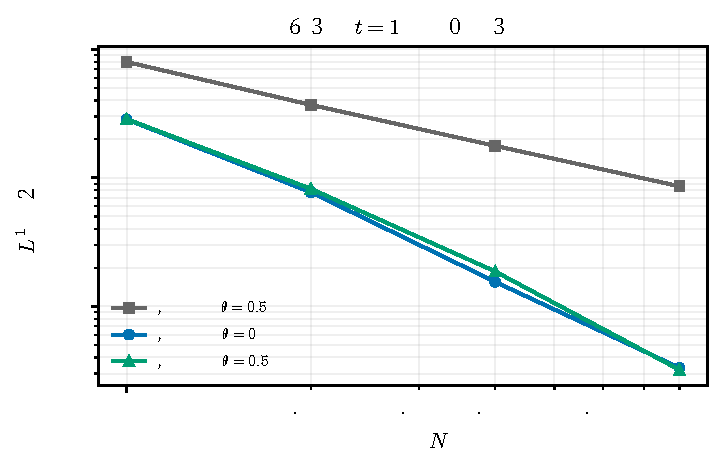
\includegraphics[width=0.72\textwidth]{convergence.pdf}
  \caption{网格收敛性（$\nu=0.01$，$\CFL=0.2$，$t=1$ 的移动粘性激波）。括号内为由首末两点估计的观测阶。}
  \label{fig:convergence}
\end{figure}

\begin{table}[htbp]
  \centering
  \caption{$L^1$ 误差随网格数的变化（$\nu=0.01$，$\CFL=0.2$，$t=1$）}
  \label{tab:convergence}
  \begin{tabular}{cccc}
    \toprule
    $N$ & 一阶，$\theta=0.5$ & MUSCL，$\theta=0$ & MUSCL，$\theta=0.5$ \\
    \midrule
    $100$ & $7.970\times10^{-3}$ & $2.854\times10^{-3}$ & $2.864\times10^{-3}$ \\
    $200$ & $3.692\times10^{-3}$ & $7.715\times10^{-4}$ & $8.213\times10^{-4}$ \\
    $400$ & $1.771\times10^{-3}$ & $1.551\times10^{-4}$ & $1.868\times10^{-4}$ \\
    $800$ & $8.588\times10^{-4}$ & $3.322\times10^{-5}$ & $3.207\times10^{-5}$ \\
    \midrule
    观测阶 & $1.07$ & $2.14$ & $2.16$ \\
    \bottomrule
  \end{tabular}
\end{table}

一阶格式的观测阶为 $1.07$，接近理论值 $1$。MUSCL 格式的观测阶为 $2.14$ 与 $2.16$，略高于 $2$。这一“超收敛”并不奇怪：本文的激波是粘性激波，过渡层是光滑的，且宽度约为 $14$ 个网格；minmod 限制器虽然会在极值点附近降低斜率，但在整个过渡层内解是单调的，重构基本保持二阶。若换成无粘激波（真正的间断），限制器会在间断处退化为一阶，观测阶通常会降到 $1$ 左右。因此，这里的二阶收敛是对“光滑粘性激波”而言的，不能直接推广到所有激波问题。

收敛性实验还有两个作用。其一，它验证了代码实现的正确性：误差随网格加密单调下降，阶数符合预期。其二，它说明在本实验的网格范围内，时间误差的常数较小、尚未主导：在 $\CFL=0.2$ 下，时间误差为 $O(\Delta t)=O(\Delta x)$，空间误差为 $O(\Delta x^2)$；MUSCL 的观测阶仍接近 $2$，说明空间误差在 $N=100$ 至 $800$ 的范围内占主导。若继续加密网格，一阶时间误差最终会使观测阶降到 $1$，因此这里的二阶收敛不能外推到任意细的网格。

\section{讨论}
\label{sec:exp-discussion}

把四组实验放在一起，可以得到如下几点认识。

第一，$\theta\le1/2$ 的稳定性判据在数值上得到了清晰验证。刚性相图的边界与理论曲线一致，最大步长的断崖与 $1/(2\theta-1)$ 的标度一致。这不是一个“大致趋势”，而是定量吻合：$\theta=0.55$ 至 $1$ 的实测步长与线性符号预测相差不超过 $1.6\%$，与渐近公式相差更小。

第二，稳定与准确是两个不同的问题。$\theta=1/2$ 是稳定性的临界点，却不是精度最优的选择；$\theta=0.25$ 在 MUSCL 格式下给出最小的 $L^1$ 误差。对于需要长时间积分的问题，$\theta=0$ 的 L-稳定性质可能比 $\theta=0.25$ 的少许精度优势更重要；对于短时间、强激波问题，$\theta=0.25$ 或 $0.5$ 可能更合适。参数选择应结合具体需求，而不是盲目追求“最稳定”或“最精确”。

第三，空间格式对精度的影响远大于 $\theta$。一阶格式的误差约为 $10^{-3}$，MUSCL 格式约为 $10^{-5}$，相差约 $1.2$ 至 $1.5$ 个数量级（$15$ 至 $28$ 倍）；而 $\theta$ 在稳定区域内只带来约 $2$ 倍的误差变化。因此，在实际计算中，优先投资空间重构与限制器，比微调 $\theta$ 更有效。

第四，数值扩散是一把双刃剑。Rusanov 通量的数值粘性 $\Delta x/2$ 在稳定性上有益（它扩大了允许的步长），在精度上有害（它增厚了激波）。在 $\nu$ 很小、网格较粗时，数值扩散可能远大于物理粘性，此时计算结果反映的主要是格式的耗散，而不是物理。本文的激波算例中，$\nu=0.01$、$\Delta x=6.25\times10^{-3}$，数值粘性约为物理粘性的 $30\%$，已经不可忽略。这是所有一阶激波捕捉格式的共同问题，也是发展高阶格式的动机。

第五，线性稳定性分析给出的是必要条件，非线性实验提供的是支持性证据。在可观测的范围内两者一致，说明本文的线性化模型抓住了主要机制；但非线性效应（限制器、激波、边界）仍然在细节上影响结果。例如，一阶格式的宽度误差几乎不随 $\theta$ 变化，而线性分析预测隐式扩散会改变高频阻尼；这说明在激波内部，Rusanov 数值扩散主导了高频行为，隐式部分的差异被掩盖。这种“理论—实验”的互补，是数值分析中常见且重要的。

\section{本章小结}

本章完成了四组数值实验，主要结论如下：
\begin{enumerate}[label=(\arabic*),leftmargin=2.4em]
  \item 刚性相图显示，$\theta\le1/2$ 时格式在 $\nu$ 从 $10^{-2}$ 到 $10^{2}$ 的范围内保持稳定；$\theta>1/2$ 时存在有限的 $\nu$ 阈值，阈值与离散条件 \eqref{eq:sawtooth-condition} 定量一致。
  \item 最大稳定步长在 $\theta=1/2$ 处发生断崖式下降；$\theta>1/2$ 时按 $\Delta x^2/[2\nu(2\theta-1)]$ 收缩，实测与线性预测相差不超过 $2\%$。
  \item 在稳定区域内，$\theta$ 对激波精度的影响是温和的；MUSCL 格式下 $\theta=0.25$ 最优，$\theta=1$ 最差，但差别不超过 $2$ 倍。空间格式的阶数才是精度的决定因素。
  \item 网格收敛实验给出一阶格式的观测阶 $1.07$、MUSCL 格式的观测阶 $2.14$ 至 $2.16$，验证了代码与理论。
\end{enumerate}
这些结果为第六章的扩展研究提供了方法基础：同样的“双变量稳定性函数 + 谱半径扫描 + 非线性验证”流程，可以直接用于 Jin--Xin 松弛系统的源项分裂。

% ==========================================================================
\chapter{Jin--Xin 松弛系统的源项分裂}
% ==========================================================================

前两章的分析建立在“对流显式、扩散隐式”的分裂之上。本章把同一套语言推广到另一类刚性系统——Jin--Xin 松弛系统。这里的刚性不再来自空间导数，而来自源项中的 $1/\varepsilon$；分裂的对象也从扩散算子变成了源项。第 \ref{sec:jinxin-model} 节介绍模型与平衡极限；第 \ref{sec:jinxin-splitting} 节给出两种源项分裂；第 \ref{sec:jinxin-stability} 节推导 $2\times2$ 放大矩阵并作谱分析；第 \ref{sec:jinxin-numerics} 节给出数值对比；第 \ref{sec:jinxin-discussion} 节讨论结果的含义。

\section{Jin--Xin 松弛系统}
\label{sec:jinxin-model}

对无粘 Burgers 方程 $u_t+f(u)_x=0$，$f(u)=u^2/2$，Jin 与 Xin 引入松弛系统\cite{jinxin1995}
\begin{equation}
  \begin{cases}
    u_t+v_x=0,\\[4pt]
    v_t+a^2u_x=-\dfrac{1}{\varepsilon}\bigl(v-f(u)\bigr),
  \end{cases}
  \label{eq:jinxin}
\end{equation}
其中 $v$ 为松弛变量，$a>0$ 为常数，$\varepsilon>0$ 为松弛参数。当 $\varepsilon\to0$ 时，源项强迫 $v\to f(u)$，第二个方程退化为 $v=f(u)$，第一个方程变为
\begin{equation}
  u_t+f(u)_x=0.
  \label{eq:equilibrium}
\end{equation}
因此，松弛系统是对原守恒律的一种逼近：它把非线性通量 $f(u)$ 替换为一个线性双曲系统加一个刚性源项。

\subsection{平衡极限与次特征条件}

对 \eqref{eq:jinxin} 作 Chapman--Enskog 展开。设 $v=f(u)+\varepsilon v_1+O(\varepsilon^2)$，代入第二个方程并保留首阶项，得
\begin{equation}
  v_1=-\bigl(f'(u)u_t+a^2u_x\bigr).
  \label{eq:chapman-enskog}
\end{equation}
再利用 $u_t=-v_x=-f(u)_x+O(\varepsilon)$，可得一阶修正。要使松弛系统在 $\varepsilon\to0$ 时稳定地收敛到 \eqref{eq:equilibrium}，特征速度 $a$ 必须不小于平衡通量的特征速度：
\begin{equation}
  a\ge\max_u|f'(u)|=\max_u|u|.
  \label{eq:subcharacteristic}
\end{equation}
这就是次特征条件。本文取 $a=1$，初始数据 $u_L=1$、$u_R=0$，因此条件恰好取等号。

松弛系统的优点是通量线性：$u$ 的通量为 $v$，$v$ 的通量为 $a^2u$。这使得我们可以直接套用有限体积的 Rusanov 通量，而不必处理非线性 Riemann 问题。代价是源项具有 $1/\varepsilon$ 的刚性，必须用隐式或渐近保持方法处理。

\subsection{线性化}

设 $\bar u$ 为常数状态，$b=f'(\bar u)=\bar u$。在 $(\bar u,f(\bar u))$ 附近线性化 \eqref{eq:jinxin}：
\begin{equation}
  \begin{pmatrix}\delta u\\ \delta v\end{pmatrix}_t
  +\begin{pmatrix}0&1\\ a^2&0\end{pmatrix}
  \begin{pmatrix}\delta u\\ \delta v\end{pmatrix}_x
  =\frac{1}{\varepsilon}
  \begin{pmatrix}0&0\\ b&-1\end{pmatrix}
  \begin{pmatrix}\delta u\\ \delta v\end{pmatrix}.
  \label{eq:jinxin-linear}
\end{equation}
源项的 Jacobian 为
\begin{equation}
  \bJ=\frac{1}{\varepsilon}
  \begin{pmatrix}0&0\\ b&-1\end{pmatrix}.
  \label{eq:source-jacobian}
\end{equation}
它有一个零特征值（对应 $u$ 的守恒模态）和一个 $-1/\varepsilon$ 的特征值（对应 $v$ 的快速松弛模态）。刚性正来自后者的模 $1/\varepsilon$。

\section{两种源项分裂}
\label{sec:jinxin-splitting}

对 \eqref{eq:jinxin} 采用 IMEX-Euler：输运项显式，源项按不同方式分裂。设 $\mu=\Delta t/\varepsilon$，并记 $\bL$ 为 Rusanov 离散后的输运算子。

\subsection{策略 A：源项全隐式}

策略 A 把整个源项放在新时刻：
\begin{equation}
  \begin{cases}
    u^{n+1}=u^n+\Delta t\,\bL_u(u^n,v^n),\\[4pt]
    v^{n+1}=v^n+\Delta t\,\bL_v(u^n,v^n)
    -\mu\left(v^{n+1}-f(u^{n+1})\right).
  \end{cases}
  \label{eq:strategy-A}
\end{equation}
整理得
\begin{equation}
  v^{n+1}=\frac{v^n+\Delta t\,\bL_v(u^n,v^n)+\mu f(u^{n+1})}{1+\mu}.
  \label{eq:strategy-A-v}
\end{equation}
由于 $u^{n+1}$ 已由第一个方程显式算出，第二个方程不需要非线性迭代；所谓“全隐式”，是指 $v^{n+1}$ 与 $f(u^{n+1})$ 都在新时刻取值。

\subsection{策略 B：仅隐式化线性刚性部分}

策略 B 把源项写成“线性刚性部分 $-$ 非线性部分”：
\begin{equation}
  -\frac{1}{\varepsilon}\bigl(v-f(u)\bigr)
  =-\frac{1}{\varepsilon}v+\frac{1}{\varepsilon}f(u).
  \label{eq:source-split}
\end{equation}
只对 $-v/\varepsilon$ 作隐式处理，$f(u)/\varepsilon$ 在旧时刻取值：
\begin{equation}
  \begin{cases}
    u^{n+1}=u^n+\Delta t\,\bL_u(u^n,v^n),\\[4pt]
    v^{n+1}=v^n+\Delta t\,\bL_v(u^n,v^n)
    -\mu v^{n+1}+\mu f(u^n).
  \end{cases}
  \label{eq:strategy-B}
\end{equation}
整理得
\begin{equation}
  v^{n+1}=\frac{v^n+\Delta t\,\bL_v(u^n,v^n)+\mu f(u^n)}{1+\mu}.
  \label{eq:strategy-B-v}
\end{equation}
与策略 A 相比，式 \eqref{eq:strategy-B-v} 只是把 $f(u^{n+1})$ 换成了 $f(u^n)$。在实现上，这一差别很小；但在稳定性上，它却是本质的。

\subsection{一个看似无害的差别}

如果不看输运项，只分析源项本身，策略 A 与 B 的放大矩阵都是
\begin{equation}
  \begin{pmatrix}1&0\\ \dfrac{\mu b}{1+\mu}&\dfrac{1}{1+\mu}\end{pmatrix},
  \label{eq:source-only}
\end{equation}
特征值为 $1$ 与 $1/(1+\mu)$。两者都稳定，且快速模态都被 $1/(1+\mu)$ 压掉。因此，\textbf{仅看源项}无法区分 A 与 B；必须把输运项与源项耦合起来，使用完整的 $2\times2$ 放大矩阵。这正是双变量稳定性函数思想在松弛系统中的体现。

\section{线性稳定性分析}
\label{sec:jinxin-stability}

\subsection{输运算子的符号}

对 \eqref{eq:jinxin} 的线性输运算符
\begin{equation}
  \bA=\begin{pmatrix}0&1\\ a^2&0\end{pmatrix},
  \label{eq:transport-matrix}
\end{equation}
采用 Rusanov 通量，其 Fourier 符号为
\begin{equation}
  \bL(\xi)=-\frac{\ii\sin\xi}{\Delta x}\bA
  -\frac{a(1-\cos\xi)}{\Delta x}\bI.
  \label{eq:transport-symbol}
\end{equation}
令
\begin{equation}
  g=c(1-\cos\xi),\qquad h=\frac{c}{a}\sin\xi,\qquad c=\frac{a\Delta t}{\Delta x},
  \label{eq:g-h}
\end{equation}
则 $\Delta t\bL(\xi)=-\bI g-\ii h\bA$。于是
\begin{equation}
  \bI+\Delta t\bL(\xi)=
  \begin{pmatrix}1-g&-\ii h\\ -\ii a^2h&1-g\end{pmatrix}.
  \label{eq:I-plus-L}
\end{equation}

\subsection{策略 A 的放大矩阵}

由 \eqref{eq:strategy-A}，先算 $u^{n+1}=u^n+\Delta t\bL_u$，再算
\begin{equation}
  (1+\mu)v^{n+1}=v^n+\Delta t\bL_v+\mu b\,u^{n+1}.
\end{equation}
写成矩阵形式：
\begin{equation}
  \bM_A=
  \begin{pmatrix}
    1-g & -\ii h\\[4pt]
    \dfrac{\mu b(1-g)-\ii a^2h}{1+\mu}
    & \dfrac{(1-g)-\ii\mu b h}{1+\mu}
  \end{pmatrix}.
  \label{eq:M-A}
\end{equation}

\subsection{策略 B 的放大矩阵}

同理，
\begin{equation}
  \bM_B=
  \begin{pmatrix}
    1-g & -\ii h\\[4pt]
    \dfrac{-\ii a^2h+\mu b}{1+\mu}
    & \dfrac{1-g}{1+\mu}
  \end{pmatrix}.
  \label{eq:M-B}
\end{equation}
两者的差别只在第二行：A 的 $(2,1)$ 元含 $\mu b(1-g)$，$(2,2)$ 元含 $-\ii\mu b h$；B 的 $(2,1)$ 元含 $\mu b$，$(2,2)$ 元没有 $\mu b h$ 项。正是这些 $O(\mu)$ 的项，在刚性极限下决定了稳定性。

\subsection{刚性极限}

令 $\mu\to\infty$，得
\begin{align}
  \bM_A^\infty&=
  \begin{pmatrix}
    1-g&-\ii h\\ b(1-g)&-\ii b h
  \end{pmatrix},
  \label{eq:M-A-inf}\\
  \bM_B^\infty&=
  \begin{pmatrix}
    1-g&-\ii h\\ b&0
  \end{pmatrix}.
  \label{eq:M-B-inf}
\end{align}
$\bM_A^\infty$ 的两行成比例，特征值为 $0$ 与 $1-g-\ii bh$。因此
\begin{equation}
  \rho(\bM_A^\infty)=|1-g-\ii bh|.
  \label{eq:rho-A}
\end{equation}
取 $b=a$，有
\begin{equation}
  |1-g-\ii ah|^2=(1-g)^2+a^2h^2
  =1-2c(1-c)(1-\cos\xi)\le1,\qquad 0\le c\le1.
  \label{eq:rho-A-bound}
\end{equation}
所以策略 A 在 $\CFL\le1$ 时稳定，且当 $c<1$ 时除 $\xi=0$ 外都有严格小于 $1$ 的衰减。这一结论与 $\mu$ 无关，说明 A 是渐近保持的：无论 $\varepsilon$ 多小，稳定性都不退化。

$\bM_B^\infty$ 的特征值满足
\begin{equation}
  \lambda^2-(1-g)\lambda+\ii bh=0.
  \label{eq:char-B}
\end{equation}
其谱半径不能写成简单的闭式。取 $b=a$，对 $\xi$ 作数值扫描，可以得到如下结果。

\begin{itemize}[leftmargin=2.2em]
  \item 当 $c\le1/3$ 时，$\rho(\bM_B^\infty)\le1$；
  \item 当 $c>1/3$ 时，$\rho(\bM_B^\infty)>1$，且超出量随 $c$ 增大而增大；
  \item 临界值 $1/3$ 与 $\mu$ 无关：在 $\mu=0.1$ 到 $10^{4}$ 的范围内，临界 CFL 稳定在 $0.33334$ 至 $0.33344$。
\end{itemize}

表 \ref{tab:jinxin-critical} 给出了不同 $\mu$ 下的临界 CFL。可以看到，即使 $\mu$ 只有 $0.1$（源项并不算“刚性”），临界值也已经降到 $1/3$。这说明策略 B 的缺陷不是“刚性太强”造成的，而是分裂结构本身造成的：把 $f(u)$ 滞后一个时刻，破坏了输运模态与源模态之间的精确平衡，产生了一个伪增长模。

\begin{table}[htbp]
  \centering
  \caption{策略 B 的临界 CFL 随 $\mu$ 的变化（谱半径扫描）}
  \label{tab:jinxin-critical}
  \begin{tabular}{lcccccc}
    \toprule
    $\mu$ & $0.1$ & $1$ & $10$ & $10^2$ & $10^3$ & $10^4$ \\
    \midrule
    $\CFL_{\rm crit}$ & $0.33344$ & $0.33335$ & $0.33334$ & $0.33334$ & $0.33334$ & $0.33334$ \\
    \bottomrule
  \end{tabular}
\end{table}

图 \ref{fig:jinxin-stability} 给出了两种策略的谱半径随 CFL 的变化。左图中，策略 A 的曲线在 $\CFL\le1$ 时都不超过 $1$，说明它稳定；右图中，策略 B 的曲线在 $\CFL>1/3$ 后迅速上升，且 $\mu$ 越大上升越快。当 $\mu\to\infty$ 时，曲线趋近于一条与 $\mu$ 无关的极限曲线，其起点正是 $1/3$。

\begin{figure}[htbp]
  \centering
  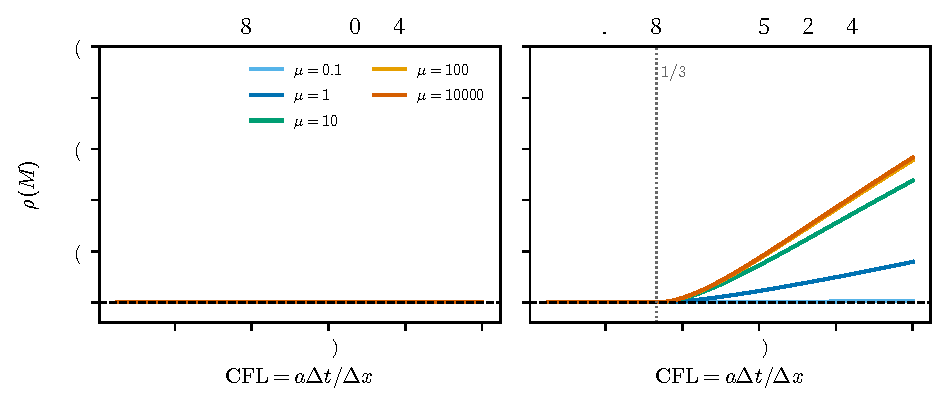
\includegraphics[width=0.96\textwidth]{jinxin_stability.pdf}
  \caption{Jin--Xin 系统两种源项分裂的谱半径。(a) 策略 A；(b) 策略 B。两图颜色对应相同的 $\mu$；虚线为 $\rho=1$，点线为 $\CFL=1/3$。}
  \label{fig:jinxin-stability}
\end{figure}

\subsection{为什么是 \texorpdfstring{$1/3$}{1/3}}

$1/3$ 的出现可以从低频展开理解。取 $b=a$，则 $bh=ah=c\sin\xi$，慢特征值近似为
\begin{equation}
  \lambda_{\rm slow}\approx\frac{\ii bh}{1-g}
  =\frac{\ii c\sin\xi}{1-c(1-\cos\xi)}.
\end{equation}
在 $\xi\to0$ 时展开：
\begin{equation}
  \lambda_{\rm slow}
  =\ii c\xi\left[1+\left(\frac{c}{2}-\frac{1}{6}\right)\xi^2+O(\xi^4)\right].
\end{equation}
方括号中的修正项在 $c=1/3$ 处变号：当 $c>1/3$ 时，低频端的模长开始超过 $1$，数值扫描显示最不稳定模态位于 $\xi/\pi\approx0.02$ 至 $0.2$，并随 $c$ 增大向高波数移动；当 $c<1/3$ 时，整个低频带的模长不超过 $1$。$c=1/3$ 正是这一低频不稳定带的起点。严格的全局证明需要对 $|\lambda|$ 作更细致的估计，本文不展开；数值扫描在 $10^{-10}$ 的精度内把临界值定在 $1/3$，足以支持后续讨论。

\section{数值实验}
\label{sec:jinxin-numerics}

在 $[-1,1]$ 上求解 \eqref{eq:jinxin}，取 $N=400$、$a=1$、$\varepsilon=10^{-4}$、$t=1$，初始数据为 Riemann 问题
\begin{equation}
  u_0(x)=\begin{cases}1,&x<0,\\0,&x>0,\end{cases}
  \qquad v_0(x)=f(u_0(x)).
  \label{eq:jinxin-riemann}
\end{equation}
精确解为以速度 $1/2$ 向右传播的激波。分别用策略 A 与 B 在 $\CFL=0.3,0.5,0.7$ 下计算，结果列于表 \ref{tab:jinxin-numerics}。

\begin{table}[htbp]
  \centering
  \caption{Jin--Xin 松弛系统的数值结果（$N=400$，$\varepsilon=10^{-4}$，$t=1$）}
  \label{tab:jinxin-numerics}
  \begin{tabular}{cccccc}
    \toprule
    策略 & $\CFL$ & 状态 & $L^1$ 误差 & $\max|u|$ & 平衡残差 \\
    \midrule
    A & $0.3$ & 稳定 & $3.292\times10^{-3}$ & $1.000$ & $3.97\times10^{-3}$ \\
    A & $0.5$ & 稳定 & $3.122\times10^{-3}$ & $1.000$ & $3.98\times10^{-3}$ \\
    A & $0.7$ & 稳定 & $2.938\times10^{-3}$ & $1.000$ & $4.12\times10^{-3}$ \\
    \midrule
    B & $0.3$ & 稳定 & $2.886\times10^{-3}$ & $1.013$ & $2.56\times10^{-2}$ \\
    B & $0.5$ & 振荡 & $2.791\times10^{-3}$ & $1.043$ & $5.67\times10^{-2}$ \\
    B & $0.7$ & 失稳 & --- & $4.45\times10^{1}$ & $7.60\times10^{2}$ \\
    \bottomrule
  \end{tabular}
\end{table}

\begin{figure}[htbp]
  \centering
  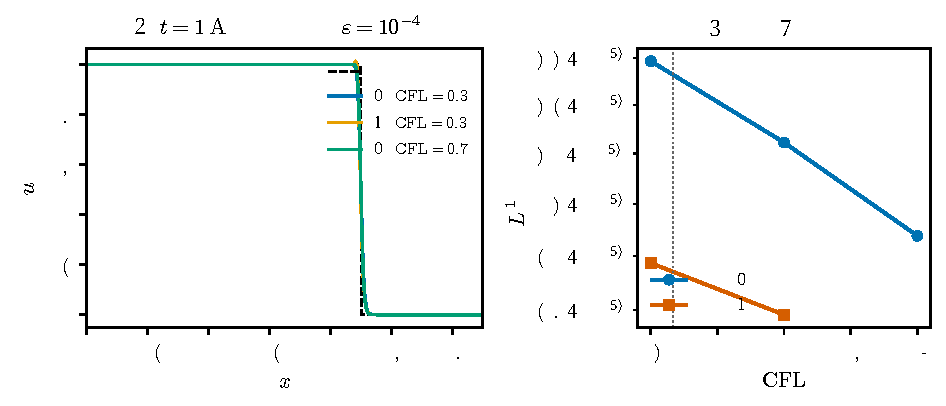
\includegraphics[width=0.94\textwidth]{jinxin_numerics.pdf}
  \caption{Jin--Xin 系统的数值对比（$\varepsilon=10^{-4}$，$t=1$）。(a) 两种策略在 $\CFL=0.3$ 的解，以及策略 A 在 $\CFL=0.7$ 的解；(b) $L^1$ 误差随 CFL 的变化。策略 B 在 $\CFL=0.7$ 时失稳，误差无定义，故其曲线止于 $\CFL=0.5$。}
  \label{fig:jinxin-numerics}
\end{figure}

表 \ref{tab:jinxin-numerics} 与图 \ref{fig:jinxin-numerics} 显示了清晰的对比：

第一，策略 A 在三个 CFL 下都稳定，$L^1$ 误差在 $2.9\times10^{-3}$ 至 $3.3\times10^{-3}$ 之间，且随 CFL 增大略有下降。这与第四章的“数值扩散随 CFL 增大而减小”的现象一致。平衡残差 $\max|v-f(u)|$ 约为 $4\times10^{-3}$，与 $L^1$ 误差同量级，说明 A 在每个时间步结束时基本把解拉回平衡流形。

第二，策略 B 在 $\CFL=0.3$ 时稳定，$L^1$ 误差甚至略小于 A（$2.886\times10^{-3}$ 对 $3.292\times10^{-3}$）；但它的平衡残差为 $2.56\times10^{-2}$，是 A 的 $6.5$ 倍。到 $\CFL=0.5$，B 的 $L^1$ 误差仍略小，但 $\max|u|$ 已增至 $1.043$，平衡残差增至 $5.67\times10^{-2}$，出现了明显的振荡；此时谱半径已略大于 $1$，只是增长较慢，尚未在 $t=1$ 内发散。到 $\CFL=0.7$，B 完全失稳，$\max|v|$ 达到 $2.3\times10^{2}$，计算中止。

第三，B 的“低 CFL 下略准”并不矛盾。B 的源项滞后一个时刻，相当于对 $f(u)$ 作了一次显式外推，这在低 CFL 下可能偶然抵消一部分数值耗散；但它破坏了平衡流形的约束，随着 CFL 增大，误差迅速积累并最终失稳。A 的平衡残差始终保持在 $4\times10^{-3}$，说明它的稳定性是有物理基础的，而不是误差抵消的结果。

\section{讨论}
\label{sec:jinxin-discussion}

\subsection{容许性与 L-稳定}

用第四章的语言，策略 A 是容许的：它在 $\CFL\le1$ 时沿刚性射线稳定，且快速模态的放大因子为 $1/(1+\mu)\to0$，因此是 L-稳定的。策略 B 不是容许的：虽然它的快速模态也被 $1/(1+\mu)$ 压掉，但慢模态的放大矩阵 $\bM_B^\infty$ 在 $\CFL>1/3$ 时谱半径大于 $1$，且这一限制不随 $\mu\to\infty$ 消失。因此，B 的失稳不是“快速模态没压住”，而是“慢模态被源项的滞后项污染了”。

\subsection{与渐近保持性质的关系}

渐近保持（AP）要求格式在 $\varepsilon\to0$ 时稳定地收敛到平衡系统的格式。策略 A 在 $\varepsilon\to0$ 时给出 $v^{n+1}\to f(u^{n+1})$，下一步的 $u$ 更新使用 $f(u^{n+1})$，因此极限格式是平衡系统的一阶显式格式。策略 B 给出 $v^{n+1}\to f(u^n)$，极限格式用的是上一步的 $f$，相当于多了一个时间步的滞后。两者都是一阶 AP，但 B 的滞后破坏了输运模态与源模态之间的平衡结构，导致 CFL 限制从 $1$ 降到 $1/3$。这说明：AP 性质本身不足以保证稳定性；分裂的结构同样重要。

\subsection{计算代价}

在本文的顺序分裂中，$u^{n+1}$ 先由显式输运算出，因此策略 A 计算 $f(u^{n+1})$ 并不比 B 计算 $f(u^n)$ 贵。两者的每步计算量几乎相同。若把源项与输运完全耦合求解，A 需要解一个非线性方程组，代价会更高；此时可以采用线性化的全隐式（Newton 一步）或 IMEX Runge--Kutta 方法。无论哪种实现，本文关于“滞后 $f(u)$ 会破坏容许性”的结论都适用。

\subsection{向粘性情形的推广}

若在 $u$ 方程中加入 $\nu u_{xx}$，则松弛系统变为
\begin{equation}
  \begin{cases}
    u_t+v_x=\nu u_{xx},\\[4pt]
    v_t+a^2u_x=-\dfrac{1}{\varepsilon}\bigl(v-f(u)\bigr).
  \end{cases}
  \label{eq:jinxin-viscous}
\end{equation}
对扩散项可以采用第三章的 $\theta$ 分裂，对源项可以采用本章的 A/B 分裂。两类刚性——扩散刚性 $1/\Delta x^2$ 与源项刚性 $1/\varepsilon$——可以分别处理，稳定性分析仍然是“双变量”的，只是变量从二维增加到三维（$z_E,z_I,\mu$）。本文不展开这一推广，但它说明了本文框架的可迁移性。

\section{本章小结}

本章把双变量稳定性函数的语言推广到 Jin--Xin 松弛系统，比较了两种源项分裂。主要结论如下：
\begin{enumerate}[label=(\arabic*),leftmargin=2.4em]
  \item 仅分析源项无法区分策略 A 与 B；必须使用包含输运耦合的 $2\times2$ 放大矩阵。
  \item 策略 A 在 $\CFL\le1$ 时稳定，且与 $\mu$ 无关；其刚性极限的特征值为 $0$ 与 $1-g-\ii bh$，模不超过 $1$。
  \item 策略 B 的临界 CFL 为 $1/3$，且该值在 $\mu=0.1$ 到 $10^{4}$ 的范围内几乎不变。B 的失稳源于 $f(u)$ 的滞后破坏了慢模态的结构。
  \item 数值实验验证了上述结论：A 在 $\CFL=0.7$ 时仍稳定，B 在 $\CFL=0.7$ 时失稳；B 在低 CFL 下虽然略准，但平衡残差随 CFL 迅速增大。
\end{enumerate}
这些结果说明，“容许分裂”不仅是扩散分裂的设计准则，也是松弛系统源项分裂的设计准则。

% ==========================================================================
\chapter{结论与展望}
% ==========================================================================

\section{主要结论}

本文以常微分方程初值问题的数值算法为主线，研究了粘性 Burgers 方程经有限体积离散后得到的刚性初值问题，系统分析了参数化 IMEX-Euler 分裂族的耦合刚性稳定性，并把相关语言推广到 Jin--Xin 松弛系统的源项分裂。主要结论可以概括为以下五点。

第一，建立了一个覆盖全显式到全隐式的单参数分裂族。通过引入 $\theta\in[0,1]$，把耗散算子按 $\theta$ 与 $1-\theta$ 的比例分配至显式与隐式部分。该族把全显式（$\theta=1$）、对半分裂（$\theta=1/2$）与全隐式（$\theta=0$）纳入同一框架，为系统比较不同分裂提供了设计空间。

第二，给出了耦合刚性稳定性的精确条件。对纯耗散情形，双变量稳定性函数沿刚性射线的值为
\begin{equation}
  R\left(-\theta x,-(1-\theta)x\right)=\frac{1-\theta x}{1+(1-\theta)x},
\end{equation}
稳定性 $|R|\le1$ 当且仅当
\begin{equation}
  (1-2\theta)x+2\ge0.
\end{equation}
因此，$\theta\le1/2$ 时格式对所有刚性稳定；$\theta>1/2$ 时仅对 $x\le2/(2\theta-1)$ 稳定。在该分裂族与纯耗散刚性极限下，这一条件既是必要的，也是充分的，且证明只用到初等代数与复平面圆盘的几何直观。对连续符号，进一步得到联合稳定条件 $\mu^2\le2d+(1-2\theta)d^2$；用刚性比 $\varepsilon=z_I/z_E$ 可把它写成 $|\varepsilon|\ge1$，而分裂族对应 $\varepsilon=(1-\theta)/\theta$。

第三，澄清了 A-稳定与 L-稳定的区别。沿刚性射线，只有 $\theta=0$ 是 L-稳定的（$R\to0$）；$0<\theta\le1/2$ 沿刚性射线稳定，但极限放大因子为 $-\theta/(1-\theta)\ne0$；$\theta=1/2$ 是临界情形，极限为 $-1$，表现为不衰减的锯齿振荡。因此，“稳定”不等于“刚性衰减”；对于需要快速压掉快模态的问题，应优先选择 $\theta=0$。

第四，完成了离散符号分析与数值验证。对一阶 Rusanov 格式，导出了网格尺度条件
\begin{equation}
  c+2(2\theta-1)r\le1\qquad(\theta>1/2),
\end{equation}
它解释了 $\theta>1/2$ 时最大步长按 $\Delta x^2/[2\nu(2\theta-1)]$ 收缩的现象。数值实验表明：刚性相图的边界与 $\theta=1/2$ 一致；$\theta=0.55$ 至 $1$ 的实测最大步长与线性预测相差不超过 $2\%$；MUSCL 格式的激波误差比一阶格式低 $15$ 至 $28$ 倍，观测收敛阶约为 $2$。

第五，把框架推广到 Jin--Xin 松弛系统。比较了源项全隐式（策略 A）与仅隐式化线性刚性部分（策略 B）两种分裂。谱分析表明，A 在 $\CFL\le1$ 时稳定，B 的临界 CFL 为 $1/3$，且该限制在 $\mu=0.1$ 到 $10^{4}$ 的范围内几乎不变。数值实验验证了 B 在 $\CFL=0.7$ 时的失稳，并揭示了 B 的平衡残差随 CFL 迅速增大的现象。

\section{局限性}

本文的分析存在以下局限，需要在后续研究中改进。

其一，稳定性分析基于线性化与冻结系数。对非线性 Burgers 方程，激波附近的系数变化、限制器的开关、边界条件等都可能影响稳定性。线性分析给出的是必要条件，非线性稳定性需要借助能量方法、TVD 性质或数值实验来补充。本文的数值实验虽然与理论一致，但没有给出严格的非线性稳定性证明。

其二，空间离散是一阶（稳定性分析）或二阶 MUSCL（精度实验），时间推进是一阶 IMEX-Euler。高阶 IMEX Runge--Kutta 方法、高阶 WENO 重构的稳定性边界可能不同；本文的结论不能直接推广到任意高阶格式。不过，“双变量稳定性函数 + 刚性射线”的框架是可迁移的，只需要把 $R(z_E,z_I)$ 换成相应格式的稳定性函数。

其三，研究对象是一维标量方程。对二维/三维系统、方程组、具有多个刚性参数的问题，稳定性函数将变成矩阵值，分析复杂度显著增加。本文的 Jin--Xin 部分已经展示了 $2\times2$ 矩阵的情形，但更一般的系统仍需进一步研究。

其四，$\theta$ 在本文中是常数。若让 $\theta$ 随时间或空间变化（自适应分裂），稳定性分析会变得更加困难；但这也可能带来更好的精度—效率平衡，是一个值得探索的方向。

其五，Jin--Xin 部分只考虑了无粘情形。粘性松弛系统的双刚性（扩散刚性 + 源项刚性）分析尚未展开；本文只给出了推广的思路，没有给出完整的定理与实验。

\section{展望}

基于本文的结果，可以在以下几个方向继续深入。

（1）\textbf{高阶格式的稳定性分析。} 把 IMEX-Euler 换成 IMEX Runge--Kutta 或 IMEX 线性多步格式，推导相应的双变量稳定性函数，研究阶数与刚性稳定性之间的权衡。特别是，能否构造在 $\theta>1/2$ 时仍保持 A-稳定的高阶格式？这需要新的分裂设计。

（2）\textbf{自适应分裂。} 让 $\theta$ 依赖于局部刚性 $|z_D|$：在刚性强的区域取较小的 $\theta$（更多隐式），在刚性弱的区域取较大的 $\theta$（更多显式）。这样可以在保证稳定性的同时降低隐式求解的规模。关键是如何设计 $\theta$ 的判据，使其既稳定又不会引入过多的数值耗散。

（3）\textbf{多维系统与算子分裂。} 把本文的框架推广到二维 Euler 方程、浅水方程等。此时扩散/粘性算子可能是张量型的，隐式求解需要多维线性系统；稳定性函数变成矩阵值，刚性射线的方向也更复杂。

（4）\textbf{非线性稳定性理论。} 用能量方法或相对熵方法证明 IMEX 格式在激波附近的有界性，而不仅仅依赖线性化。这将为“容许分裂”提供更坚实的理论基础。

（5）\textbf{与其他刚性处理方法的比较。} 除了 IMEX，还有指数积分、隐式—显式龙格—库塔、Rosenbrock 方法等。把本文的双变量稳定性语言与这些方法比较，可以更全面地理解“刚性分裂”的共性与差异。

（6）\textbf{软件实现与教学。} 本文的代码结构清晰、依赖少，适合作为数值 PDE 课程的教学案例。后续可以把它整理为一个开源教学包，包含更丰富的算例、可视化与自动稳定性分析工具。

总之，本文的工作是一个起点：它把“容许分裂”“双变量稳定性函数”“耦合刚性极限”“L-稳定”这套语言，落实为一个可以计算、可以作图、可以用数值实验检验的流程。希望这一流程能够为更复杂的双曲守恒律与刚性松弛系统的研究提供帮助。


\appendix
% ==========================================================================
\chapter{核心代码与复现说明}
% ==========================================================================

本附录给出论文核心代码的结构与关键片段。完整代码位于配套的 \texttt{Code} 文件夹（其下的 \texttt{Undergraduate Thesis Code} 子文件夹），数据位于 \texttt{data} 子文件夹，图片位于 \texttt{figures} 子文件夹。

\section{代码结构}

\begin{table}[htbp]
  \centering
  \small
  \caption{代码文件与功能}
  \label{tab:code-files}
  \begin{tabularx}{\textwidth}{lX}
    \toprule
    文件 & 功能 \\
    \midrule
    \texttt{burgers\_imex.py} & 有限体积离散、Rusanov 通量、MUSCL/minmod、IMEX-Euler \\
    \texttt{stability\_analysis.py} & 双变量稳定性函数、圆盘/相图、联合稳定域、离散符号 \\
    \texttt{run\_burgers\_experiments.py} & 刚性相图、最大步长、激波精度、收敛性 \\
    \texttt{plot\_results.py} & 从缓存数据绘制论文图 \\
    \texttt{jinxin.py} & Jin--Xin 松弛系统、两种源项分裂、谱分析 \\
    \texttt{run\_jinxin\_experiments.py} & 谱半径扫描、临界 CFL、数值对比 \\
    \texttt{stiff\_ode\_example.py} & 第二章刚性 ODE 算例 \\
    \bottomrule
  \end{tabularx}
\end{table}

\clearpage
\section{IMEX-Euler 的时间推进}

下面的片段对应 \texttt{burgers\_imex.py} 中的核心循环。矩阵 $\bA=\bI-(1-\theta)\nu\Delta t\bD$ 只分解一次，随后每步用三角回代求解。

\begin{lstlisting}[language=Python,caption={IMEX-Euler 时间推进的核心循环}]
c = (1.0 - theta) * nu * dt / dx**2
main = np.full(N, 1.0 + 2.0 * c)
off = np.full(N - 1, -c)
A = diags([off, main, off], [-1, 0, 1], format="csc")
lu = splu(A)

for n in range(nsteps):
    conv = rhs_convective(u, grid, bcl, bcr, order=order)
    lap = laplacian(u, grid, bcl, bcr)
    rhs = u + dt * (conv + theta * nu * lap)
    rhs[0] += c * bcl
    rhs[-1] += c * bcr
    u = lu.solve(rhs)
\end{lstlisting}

\section{双变量放大因子}

\begin{lstlisting}[language=Python,caption={离散符号与放大因子}]
def amplification(xi, dt, nu, theta, a, dx):
    lam_c = (-1j * a * np.sin(xi) / dx
             - abs(a) * (1.0 - np.cos(xi)) / dx)
    lam_d = -2.0 * (1.0 - np.cos(xi)) / dx**2
    z_e = dt * (lam_c + theta * nu * lam_d)
    z_i = dt * (1.0 - theta) * nu * lam_d
    return (1.0 + z_e) / (1.0 - z_i)
\end{lstlisting}

\section{Jin--Xin 源项更新}

\begin{lstlisting}[language=Python,caption={策略 A 与策略 B 的源项更新}]
du, dv = transport_rhs(u, v, grid.dx, a, uL, uR)
u_new = u + dt * du
if strategy == "A":
    v_new = (v + dt * dv + mu * f_burgers(u_new)) / (1.0 + mu)
elif strategy == "B":
    v_new = (v + dt * dv + mu * f_burgers(u)) / (1.0 + mu)
\end{lstlisting}

\section{谱半径扫描}

\begin{lstlisting}[language=Python,caption={策略 B 刚性极限的谱半径}]
g = cfl * (1.0 - np.cos(xi))
h = (cfl / a) * np.sin(xi)
M = np.array([[1.0 - g, -1j * h], [b, 0.0]])
rho = np.max(np.abs(np.linalg.eigvals(M)))
\end{lstlisting}

\section{复现步骤}

代码依赖 Python 3.10 以上版本、NumPy、SciPy 与 Matplotlib。为避免污染系统环境，可将依赖安装到本地目录：

\begin{lstlisting}[language=bash,caption={安装依赖}]
cd "Code/Undergraduate Thesis Code"
python3 -m pip install --target .pylibs \
    --break-system-packages numpy scipy matplotlib
\end{lstlisting}

然后依次运行：

\begin{lstlisting}[language=bash,caption={生成图片与数据}]
cd "Code/Undergraduate Thesis Code"
export PYTHONPATH=.:.pylibs
export MPLCONFIGDIR=/tmp/mplconfig
python3 stability_analysis.py
python3 run_burgers_experiments.py all
python3 run_jinxin_experiments.py
python3 plot_results.py
\end{lstlisting}

全部实验在普通笔记本电脑上约需数分钟。随机数未使用，结果可完全复现。


\backmatter
\printbibliography[heading=bibintoc,title={参考文献}]

\chapter*{\texorpdfstring{致\quad 谢}{致谢}}
\addcontentsline{toc}{chapter}{致谢}
\markboth{致谢}{}

本论文的完成，离不开许多人的帮助与支持。

首先感谢我的指导教师。从选题的反复讨论，到稳定性证明的逐行推敲，再到数值实验的设计与论文的修改，老师都倾注了大量心血。老师严谨的治学态度、对数学图像的敏锐把握，以及“先把问题想清楚，再动手写代码”的研究习惯，使我受益终身。在论文遇到困难时，老师总是耐心地帮我梳理思路，鼓励我从最简单的模型出发，逐步逼近问题的本质。

感谢基础科学学院各位任课教师。偏微分方程、数值分析、常微分方程等课程为我打下了必要的基础；老师们在课堂上的推导与例题，常常成为我理解新问题的钥匙。特别感谢在开题与中期检查中提出宝贵意见的各位老师，他们的建议使论文的结构更加清晰，论证更加严谨。

感谢同窗与朋友们。与他们在讨论班、自习室和线上的交流，让我少走了许多弯路。无论是一个公式的核对，还是一段代码的调试，抑或是在焦虑时的相互鼓励，这些都是我本科阶段珍贵的记忆。

感谢我的家人。他们始终尊重我的选择，在我遇到挫折时给予无条件的支持与信任。没有他们的理解与陪伴，我无法安心完成学业。

最后，感谢在百忙之中评阅本文的各位专家。文中的疏漏与不足，恳请各位老师批评指正。


\end{document}
